%!TEX root = ../thesis.tex
%*******************************************************************************
%****************************** Second Chapter *********************************
%*******************************************************************************

\chapter{Data Processing and Splitting}
\label{chap:data}
\ifpdf
    \graphicspath{{DataChapter/Figs/Raster/}{DataChapter/Figs/PDF/}{DataChapter/Figs/}}
\else
    \graphicspath{{DataChapter/Figs/Vector/}{DataChapter/Figs/}}
\fi



\section{Processing}
\subsection{Normalisation}

Count data from amplicon sequencing display a very high degree of variability in total read counts per sample \cite{inadmissible_rareying}. A histogram, Figure \ref{fig:counthistogram}, of the samples' total count reads for our data exemplifies this variability. The sums range from 17 to 219113, with a median and mean of 63672 and 77152 respectively. This much variation between samples makes it hard to identify which OTUs' difference in abundance between samples is significant and also might negatively impact the performance of the classifiers. 
 
 The increased variation comes from a systematic variability affecting multiple samples and OTUs in a similar manner. Sources of such variability can be the inconsistencies in DNA extraction and handling of samples,  a varying quality of sequencing runs \cite{pereira_comparison_2018}, and other PCR-specific amplification biases (like primer mismatch, GC-content etc.) \cite{abundance_nodate,krehenwinkel_estimating_2017}.
 
 Furthermore, these biases can cause the distribution of read counts obtained from high-throughput amplicon sequencing to diverge significantly from the actual distribution of species abundances in the same samples. The Pearson correlation between read and species frequencies is close to zero \cite{edgar_unbias:_2017}.
 
 The removal of this Systematic Variability is called \textit{Normalisation} and it's original aim in the bioinformatics literature is to increase the statistical power and false positive rates of differential abundance analysis \footnote{Differential abundance analysis aims at finding OTUs (or genes in the case of metagenomic studies) whose variation between groups of samples (e.g. black and white water river samples) is statistically significant.}. We will be testing if normalisation methods have any effect on the classifiers' scores.
 
 A normalisation method that produced promising results in differential analysis on datasets similar to ours is Cumulative sum scaling (CSS). This method is an extension to the quantile normalisation approach which divided read counts by the $Q$th percentile of each sample’s non-zero count distribution. CSS determines that percentile using a data-driven approach\cite{css_diff_abund}.
 
 To illustrate how normalisation methods work we define $X_{i,j}$ as the read counts of sample  $i =1,...,n$ and OTU $j=1,...,p$. The normalisation factor of the total sum scaling (TSS) method is found by summing the read counts in a sample $i$:
 \begin{equation}
 	N_i = \sum_{j=1}^{p} X_{ij}.
 \end{equation}
Then the counts in row $i$ of the read matrix $X$ are divided by the factor $N_i$. TSS is the most commonly used method of normalisation but it has been shown to introduce biases in differential analysis estimates \cite{bullard_evaluation_2010}.

Quantile scaling computes the normalisation factor by taking into account how OTU total counts (for all samples) vary, and choosing a percentile that produces desirable properties (such as robustness from highly abundant OTUs).
The scaling factor is defined as:
\begin{align}
	N_i &= \underset{ j \in G}{ Q\text{th quantile}} \  X_{ij}\\
	G  &= \left\{ j : \sum_{i = 1}^{n} X_{ij} > 0\right\}.
\end{align}

 
\begin{figure}[htb]
\centering
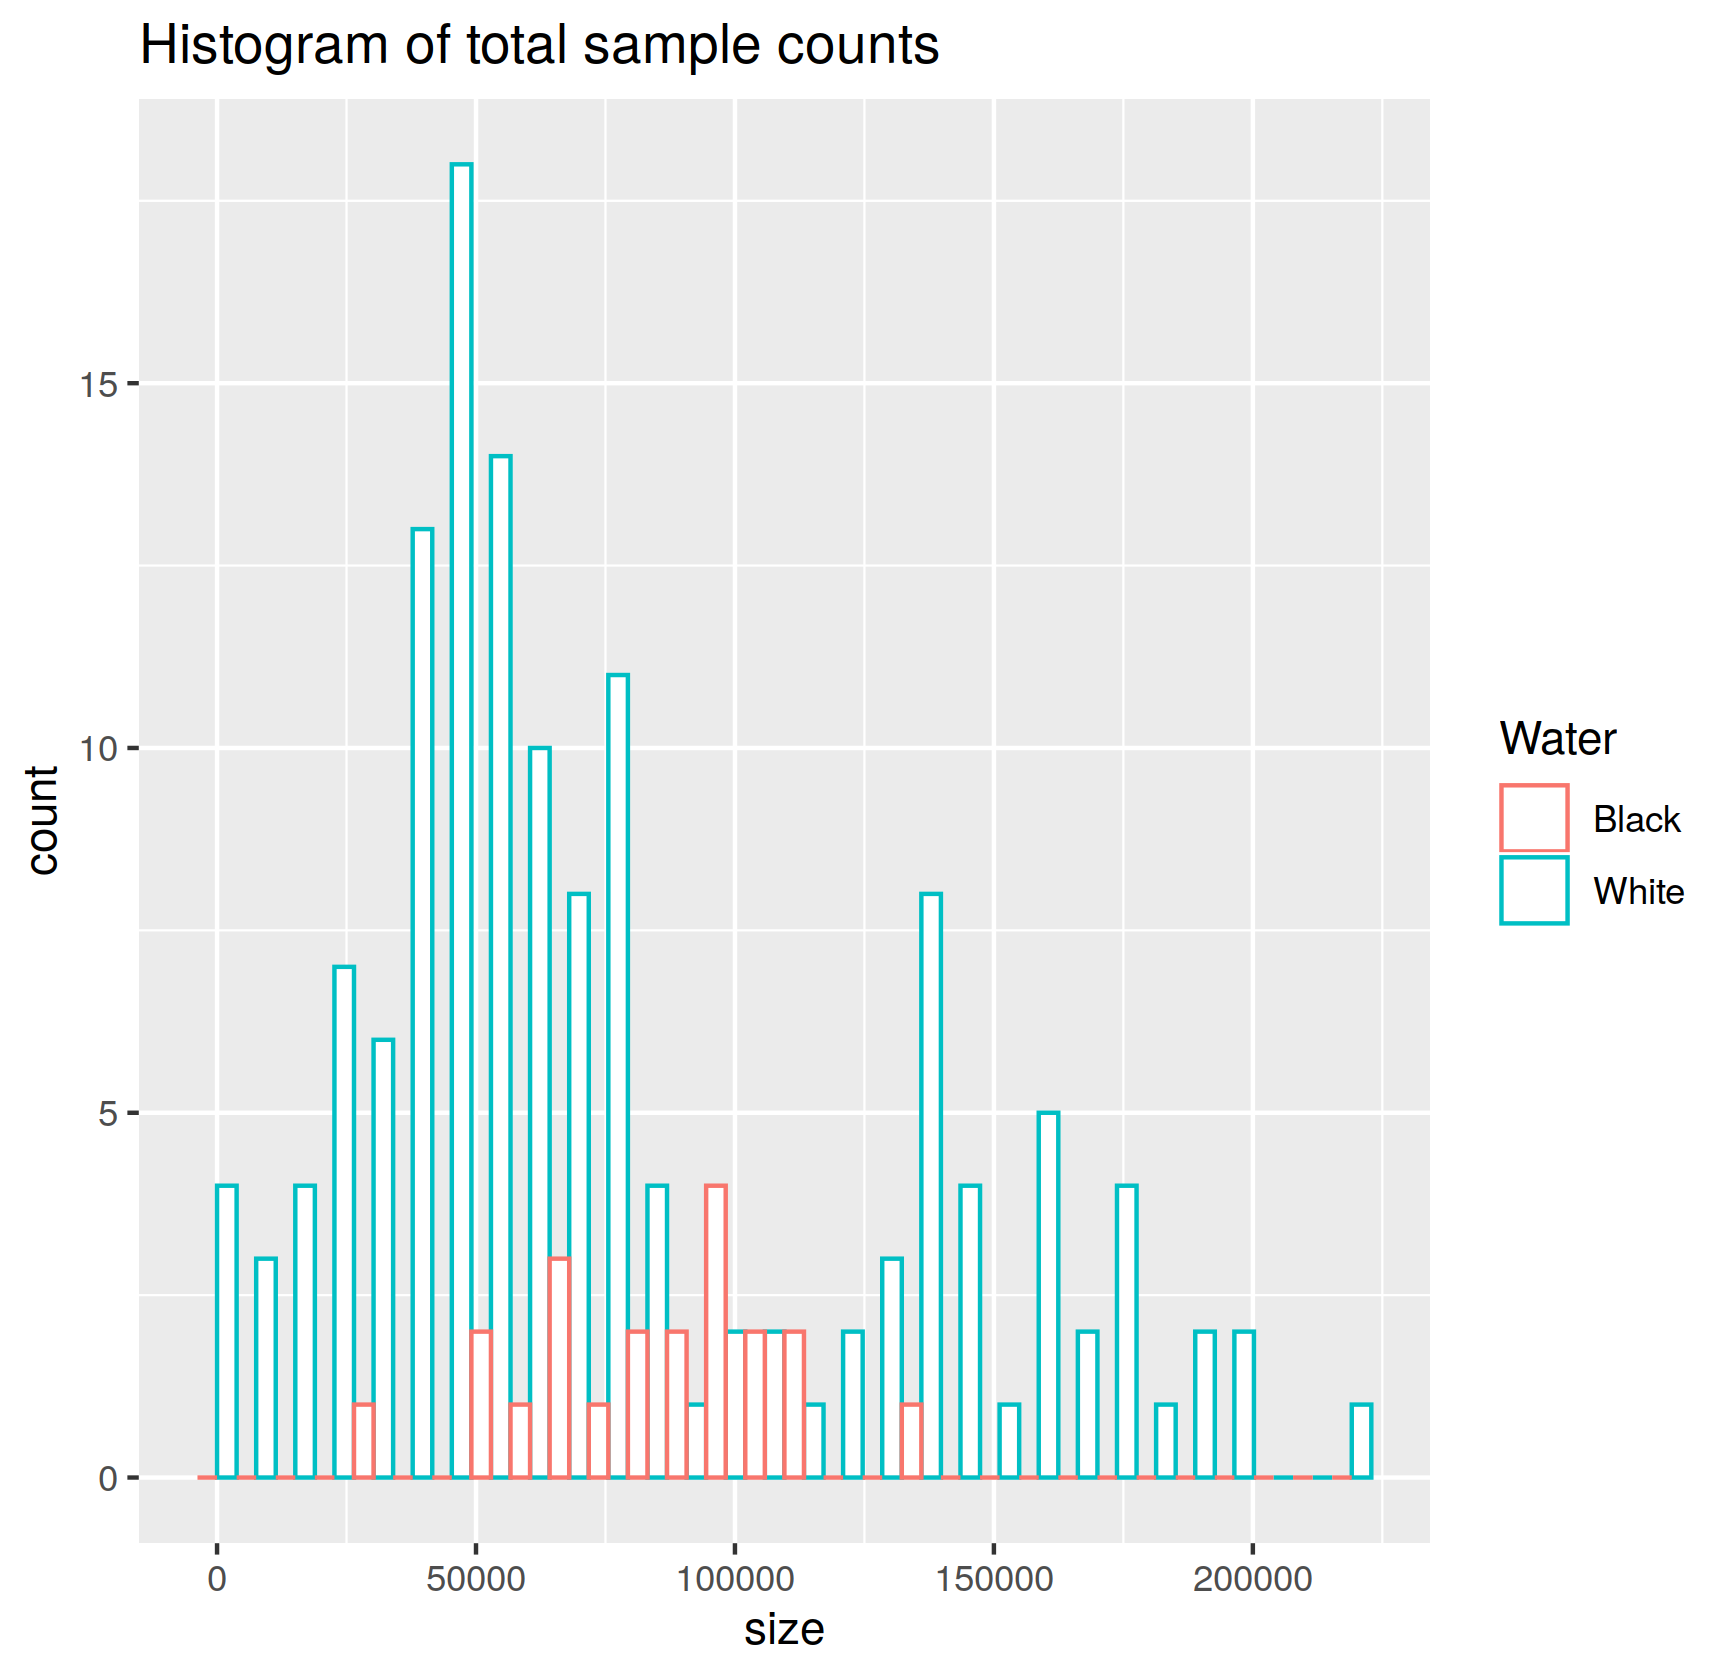
\includegraphics[width = 0.7\textwidth]{histogramofcountdata}
\caption{Histogram of the sum of OTU counts of each sample. The cyan colour represents white water samples and the red colour black water samples.}
\label{fig:counthistogram}
\end{figure}

CSS normalisation involves the calculation of a data-driven quantile 
We define the $l$th quantile of sample $i$ as $q_i^l$, which means that $l$ OTUs have a read count lower than $q_i^l$. Also we define the sum of counts per samples $i$ up to the $l$th quantile as
\begin{equation}
	s_{i}^{l}=\sum_{j|X_{ij} \leq q_{i}^{l}} X_{ij}.
\end{equation} 
With this notation, the total sum normalising factor is given by $N_i = s_i^p$ (where $p$ is the total number of OTUs). CSS chooses a value $\hat{l} \leq p$ using a data driven approach to calculate the scaling factor ($N_i = s_i^{\hat{l}}$) for each sample and get normalised counts.
In particular, the quantile $\hat{l}$ for the threshold $q_i^{\hat{l}}$ is chosen  to be the smallest value where the median absolute deviation of sample-specific quantiles $q_i^l$ from a reference point (the median quantile $q_i^l$ across all samples) shows high instability. \cite{css_diff_abund}.
% web

% CSS + LOG histograms 
\begin{figure}[h]
	\centering
	\begin{subfigure}{0.4\textwidth}
		\centering
		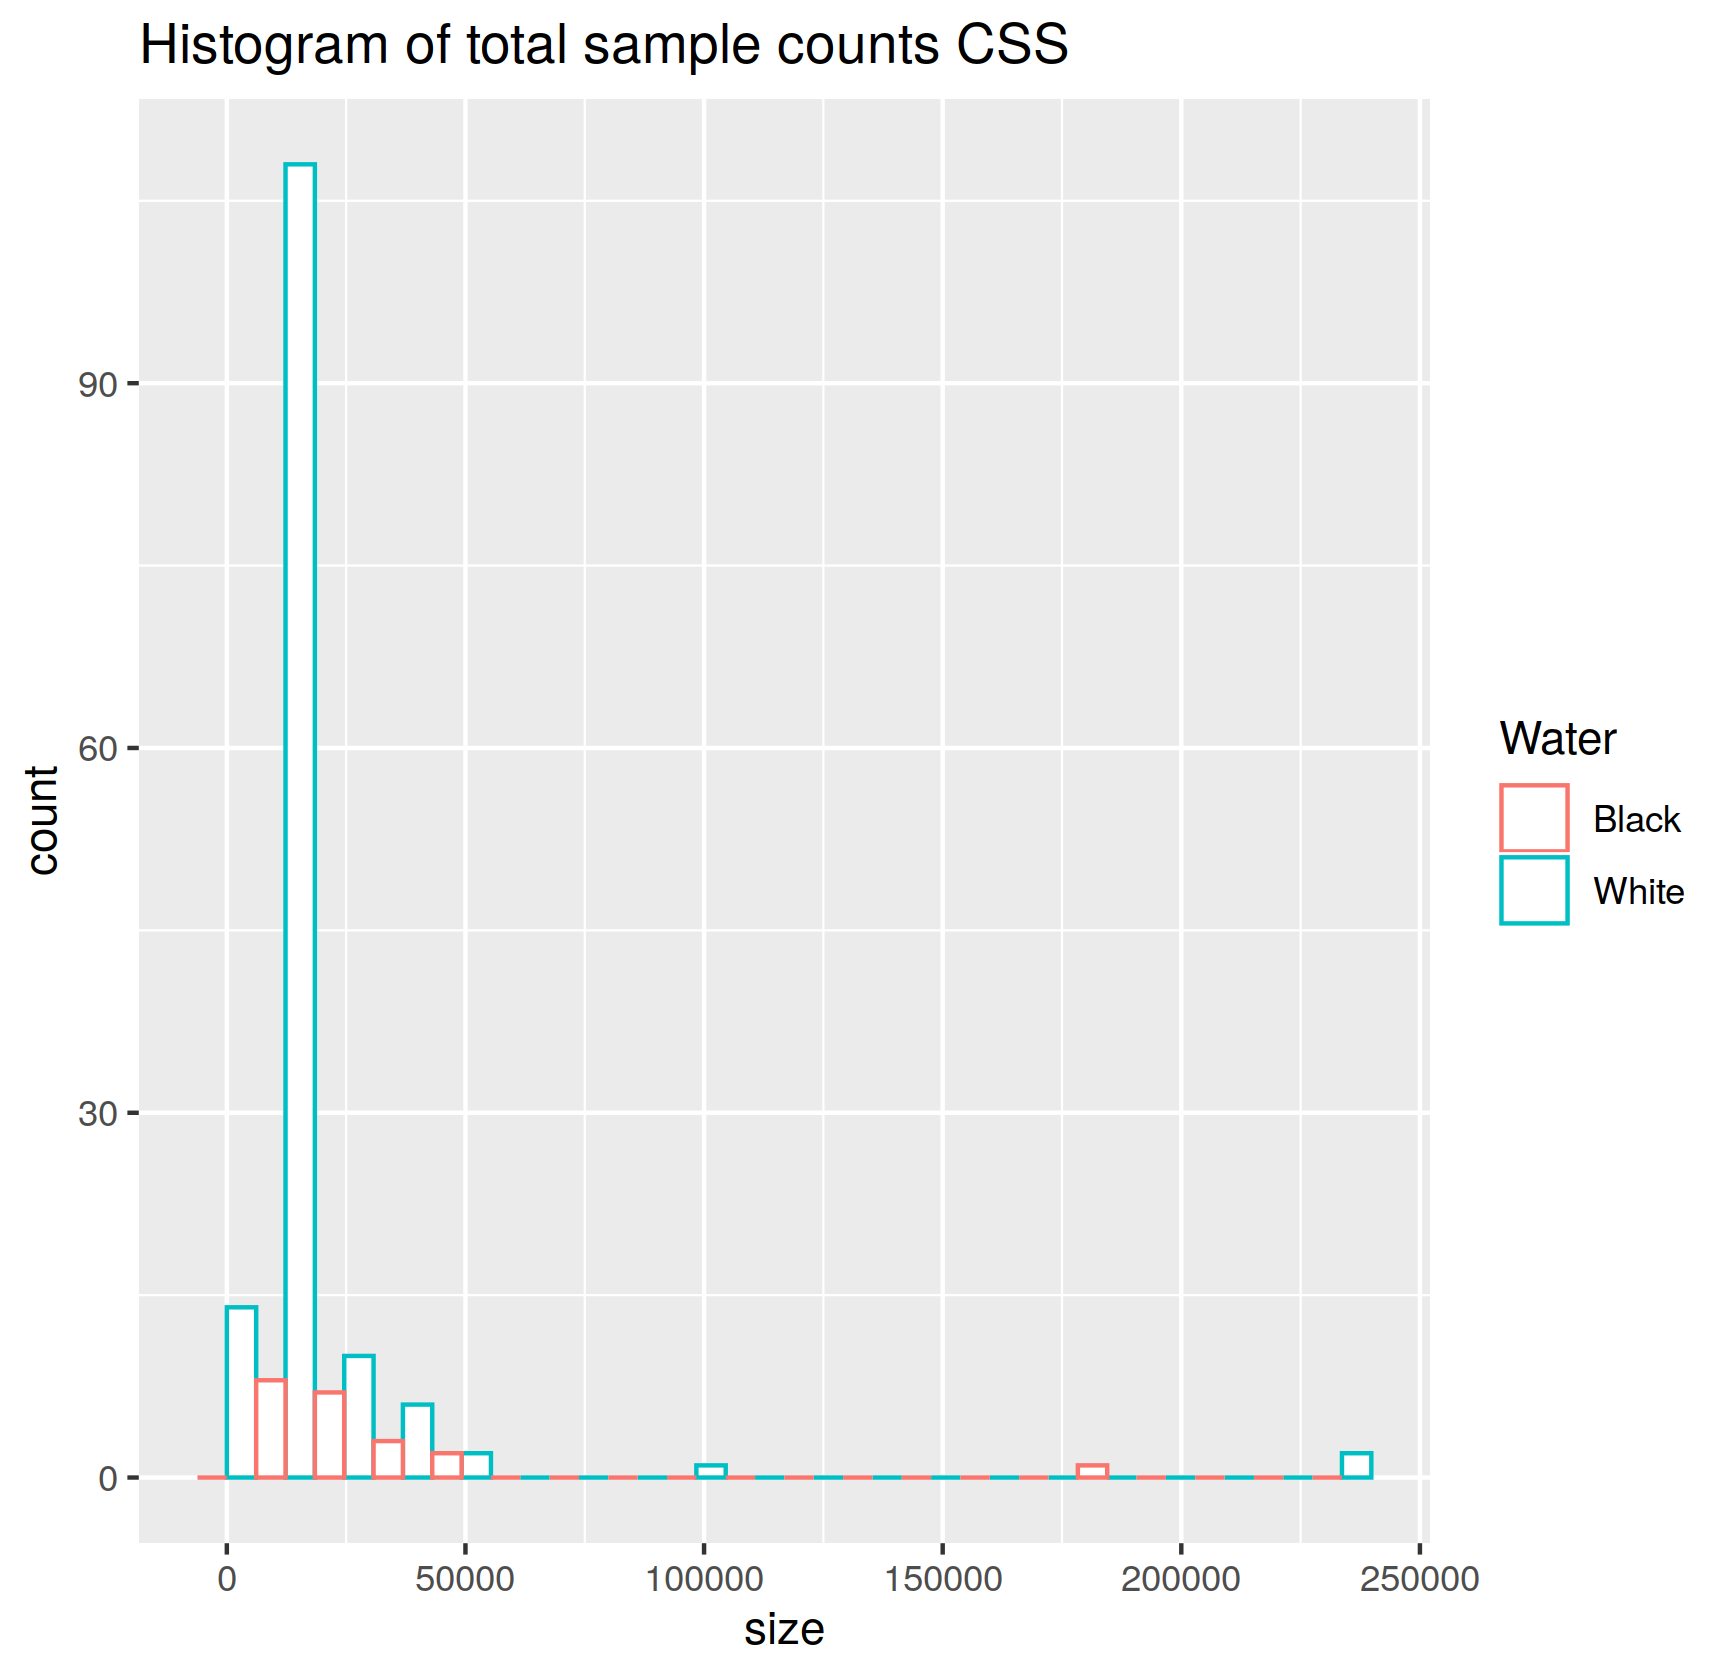
\includegraphics[width = \textwidth]{histogramofcountdatacss}
		\caption{}
		\label{fig:histcss}
	\end{subfigure}
	\begin{subfigure}{0.4\textwidth}
	\centering
	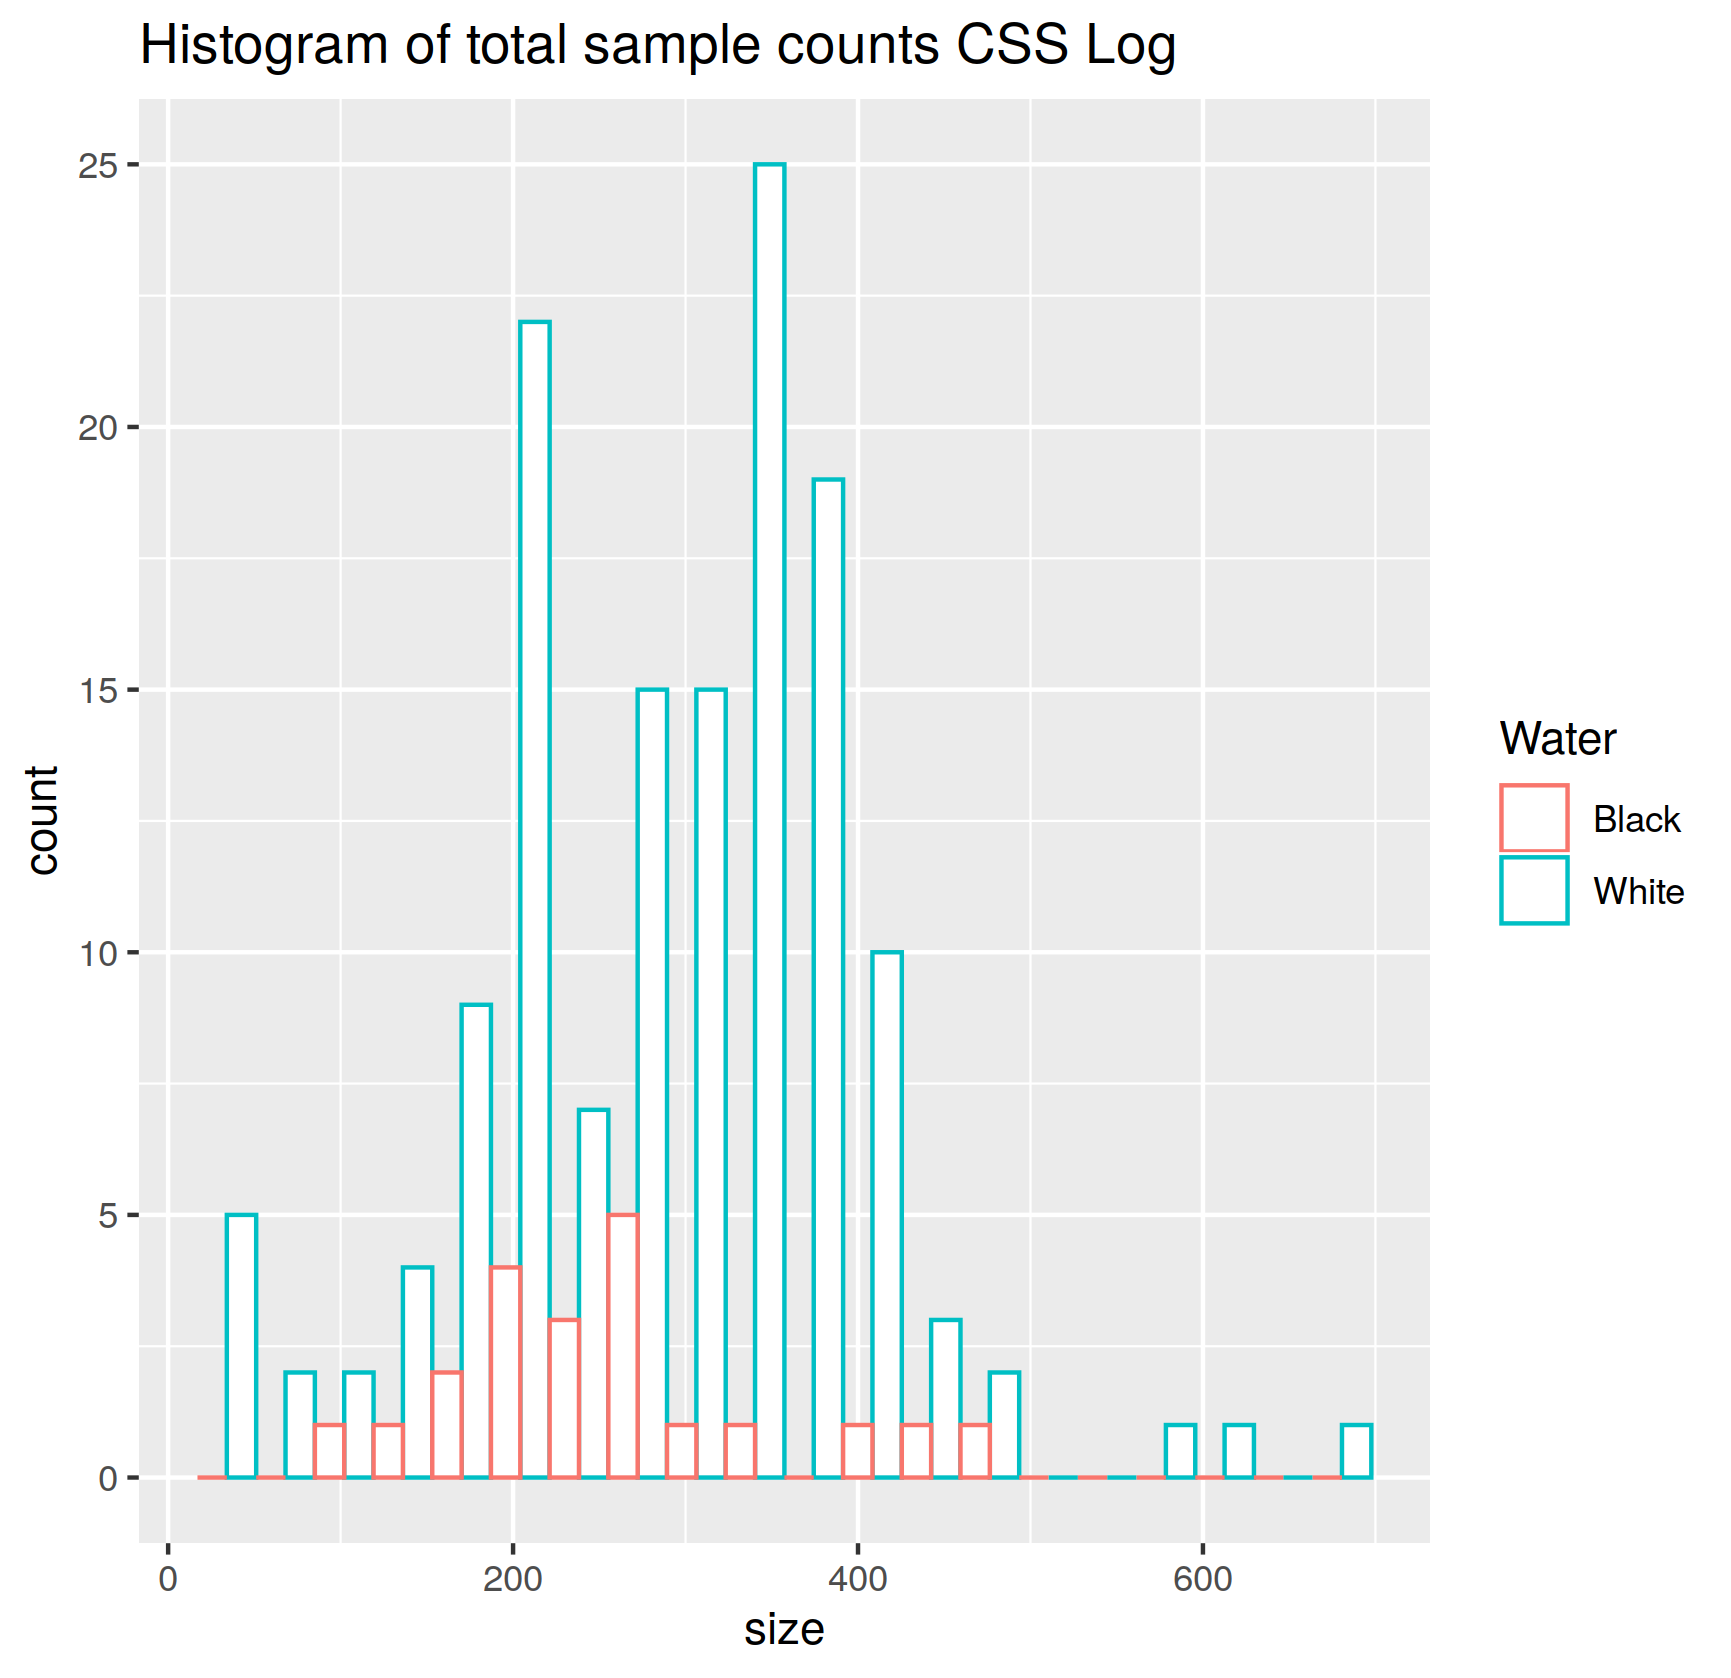
\includegraphics[width = \textwidth]{histogramofcountdatacsslog}
	\caption{}
	\label{fig:histcsslog}
	\end{subfigure}
	\caption{Histogram of the read counts per sample after \ref{fig:histcss} CSS normalisation and with \ref{fig:histcsslog} a $log_2$ transformation. The cyan colour represents white water samples and the red colour black water samples. }
\end{figure}


After applying the CSS normalisation, the variation of read counts per samples drops significantly (except for some samples whose total read counts increase, see Figure \ref{fig:histcss}). Applying a $log_2$ transformation to the data after normalising reduces the variation drops even more (see Figure \ref{fig:histcsslog}). Furthermore, using Principal coordinate analysis and Non-metric multidimensional scaling (Figure \ref{fig:pcoa12otucss} and \ref{fig:nmds12otucss} respectively) ordination on the normalised data separates white and black water samples better than if the normalisation was not applied\footcite{These methods are similar to Principal Components Analysis in that they reduce the dimensions of the data. They will be explained in the next Chapter.}. However, doing the same on the $log_2$ transformed data does not have the same effect.

\begin{figure}[h]
	\centering
	\begin{subfigure}{0.4\textwidth}
		\centering
		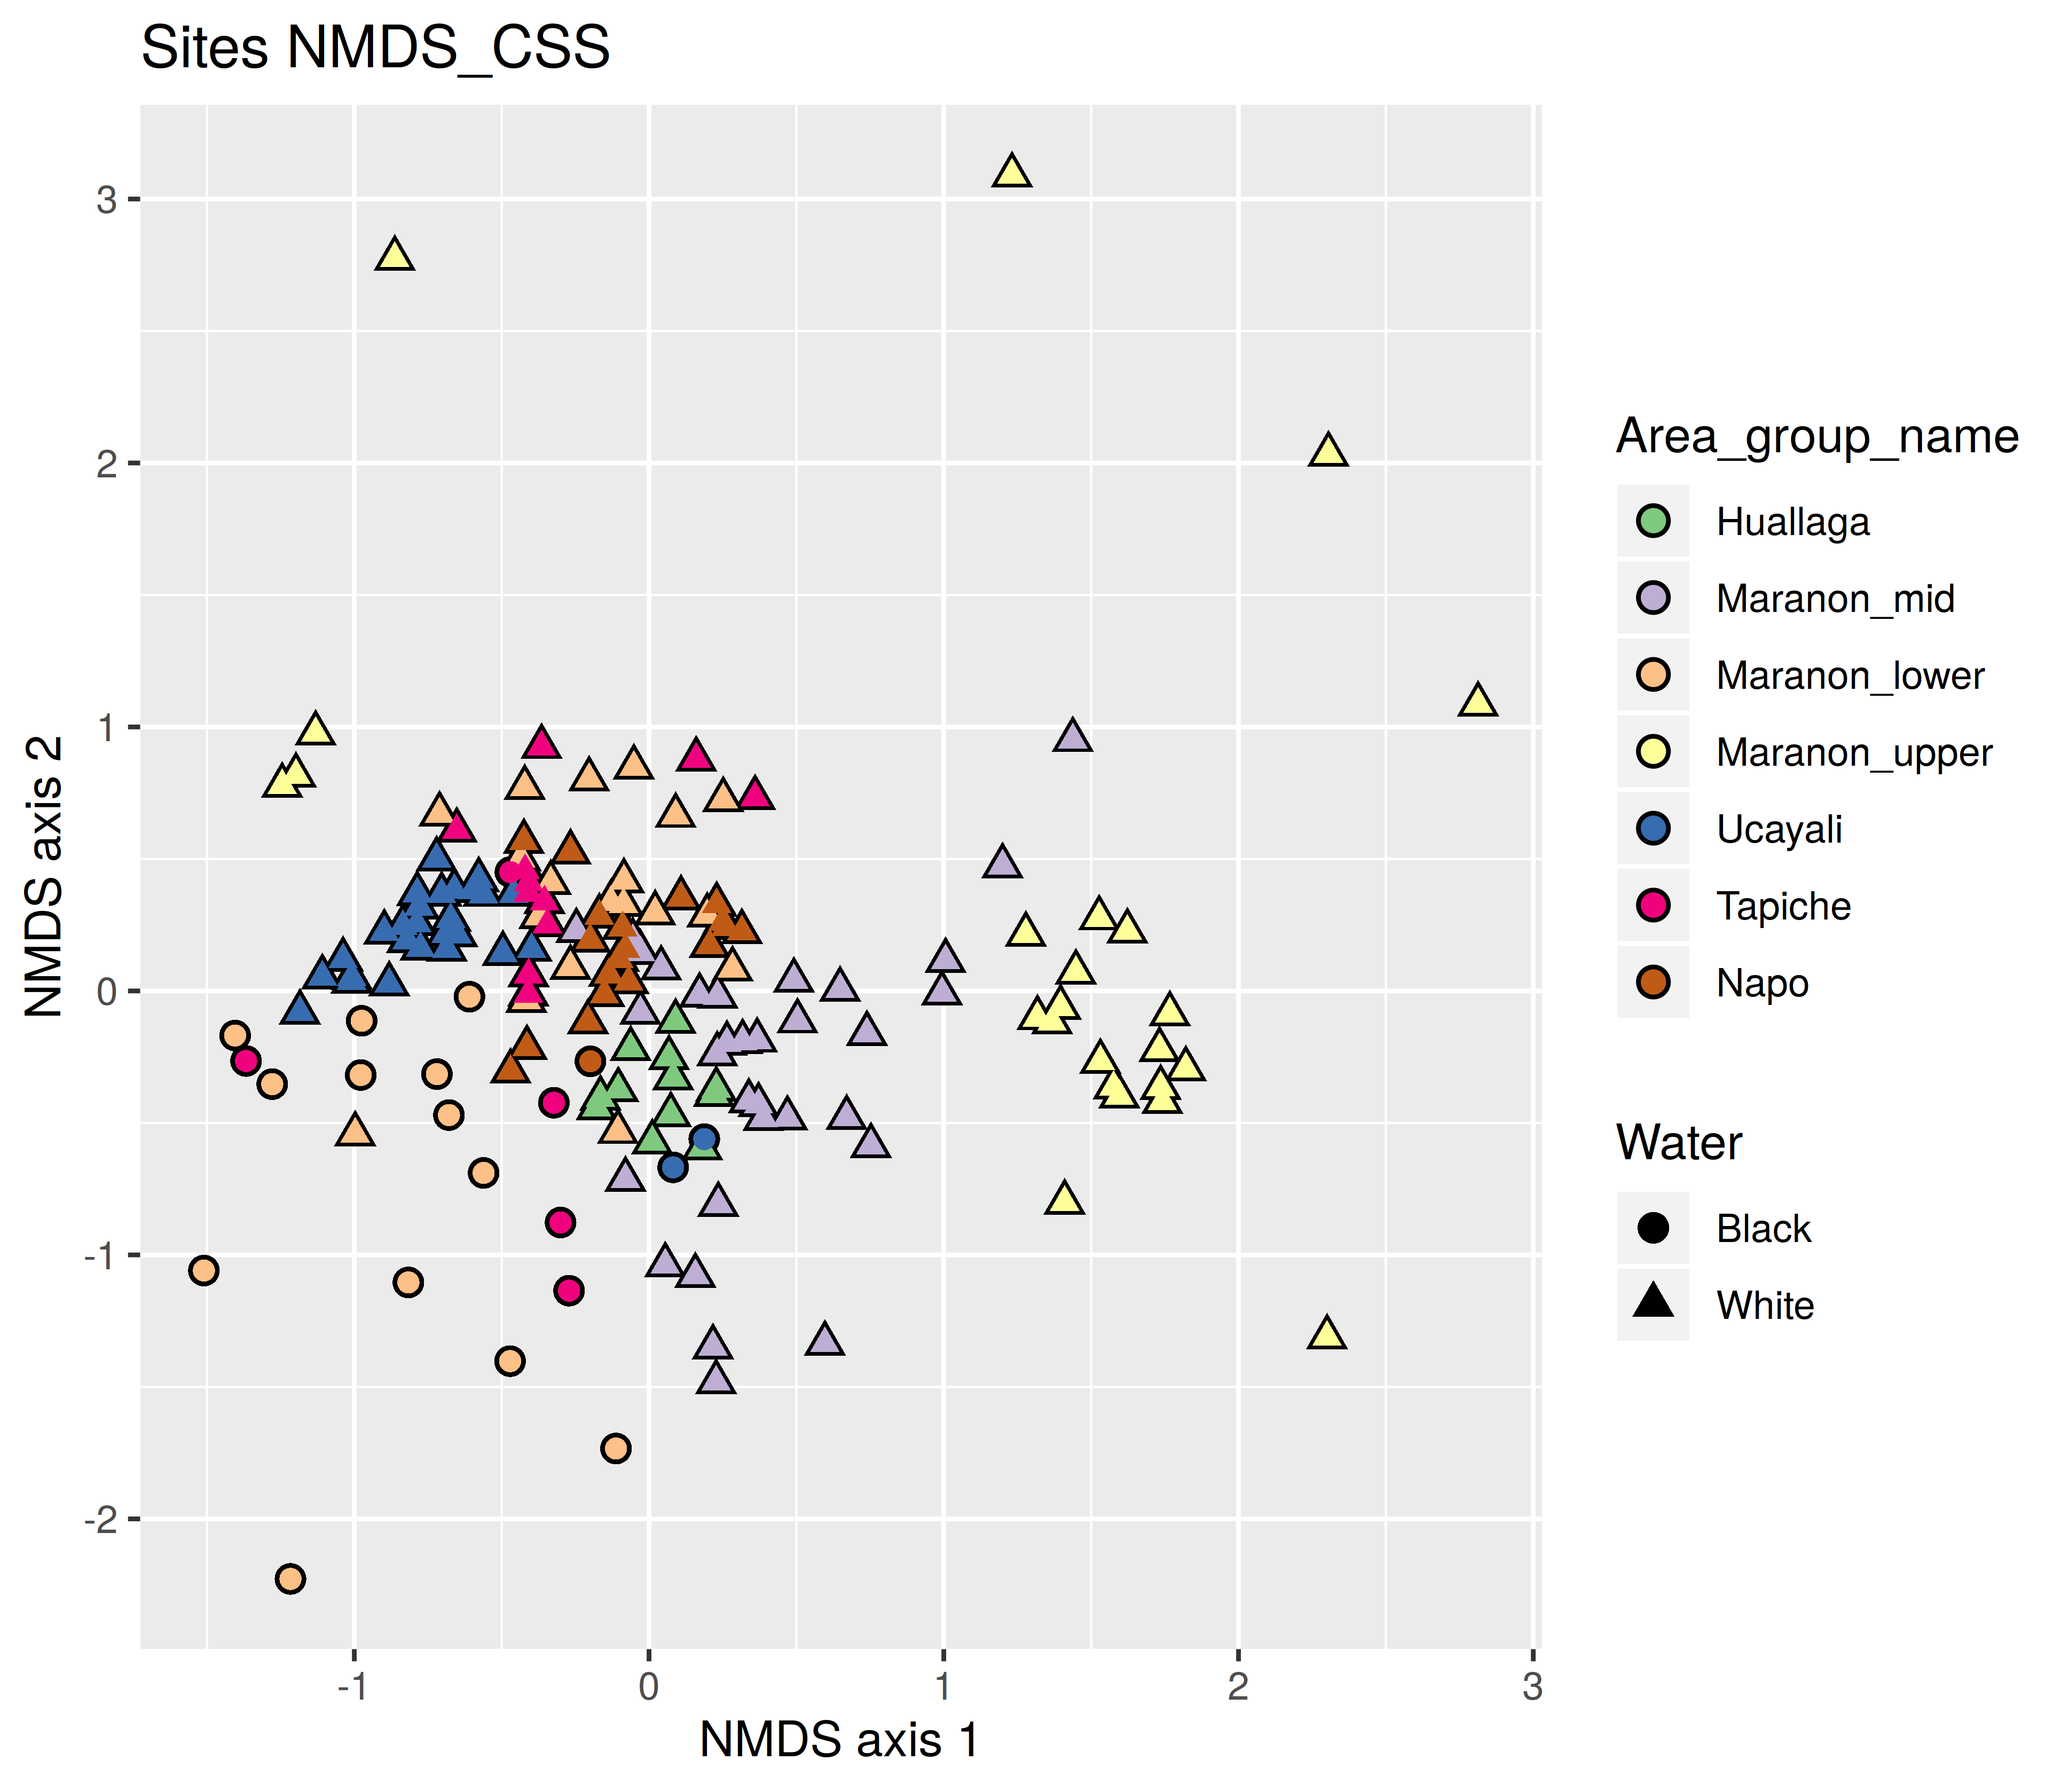
\includegraphics[width = \textwidth]{nmds12otucss}
		\caption{}
		\label{fig:nmds12otucss}
	\end{subfigure}
	\begin{subfigure}{0.4\textwidth}
		\centering
		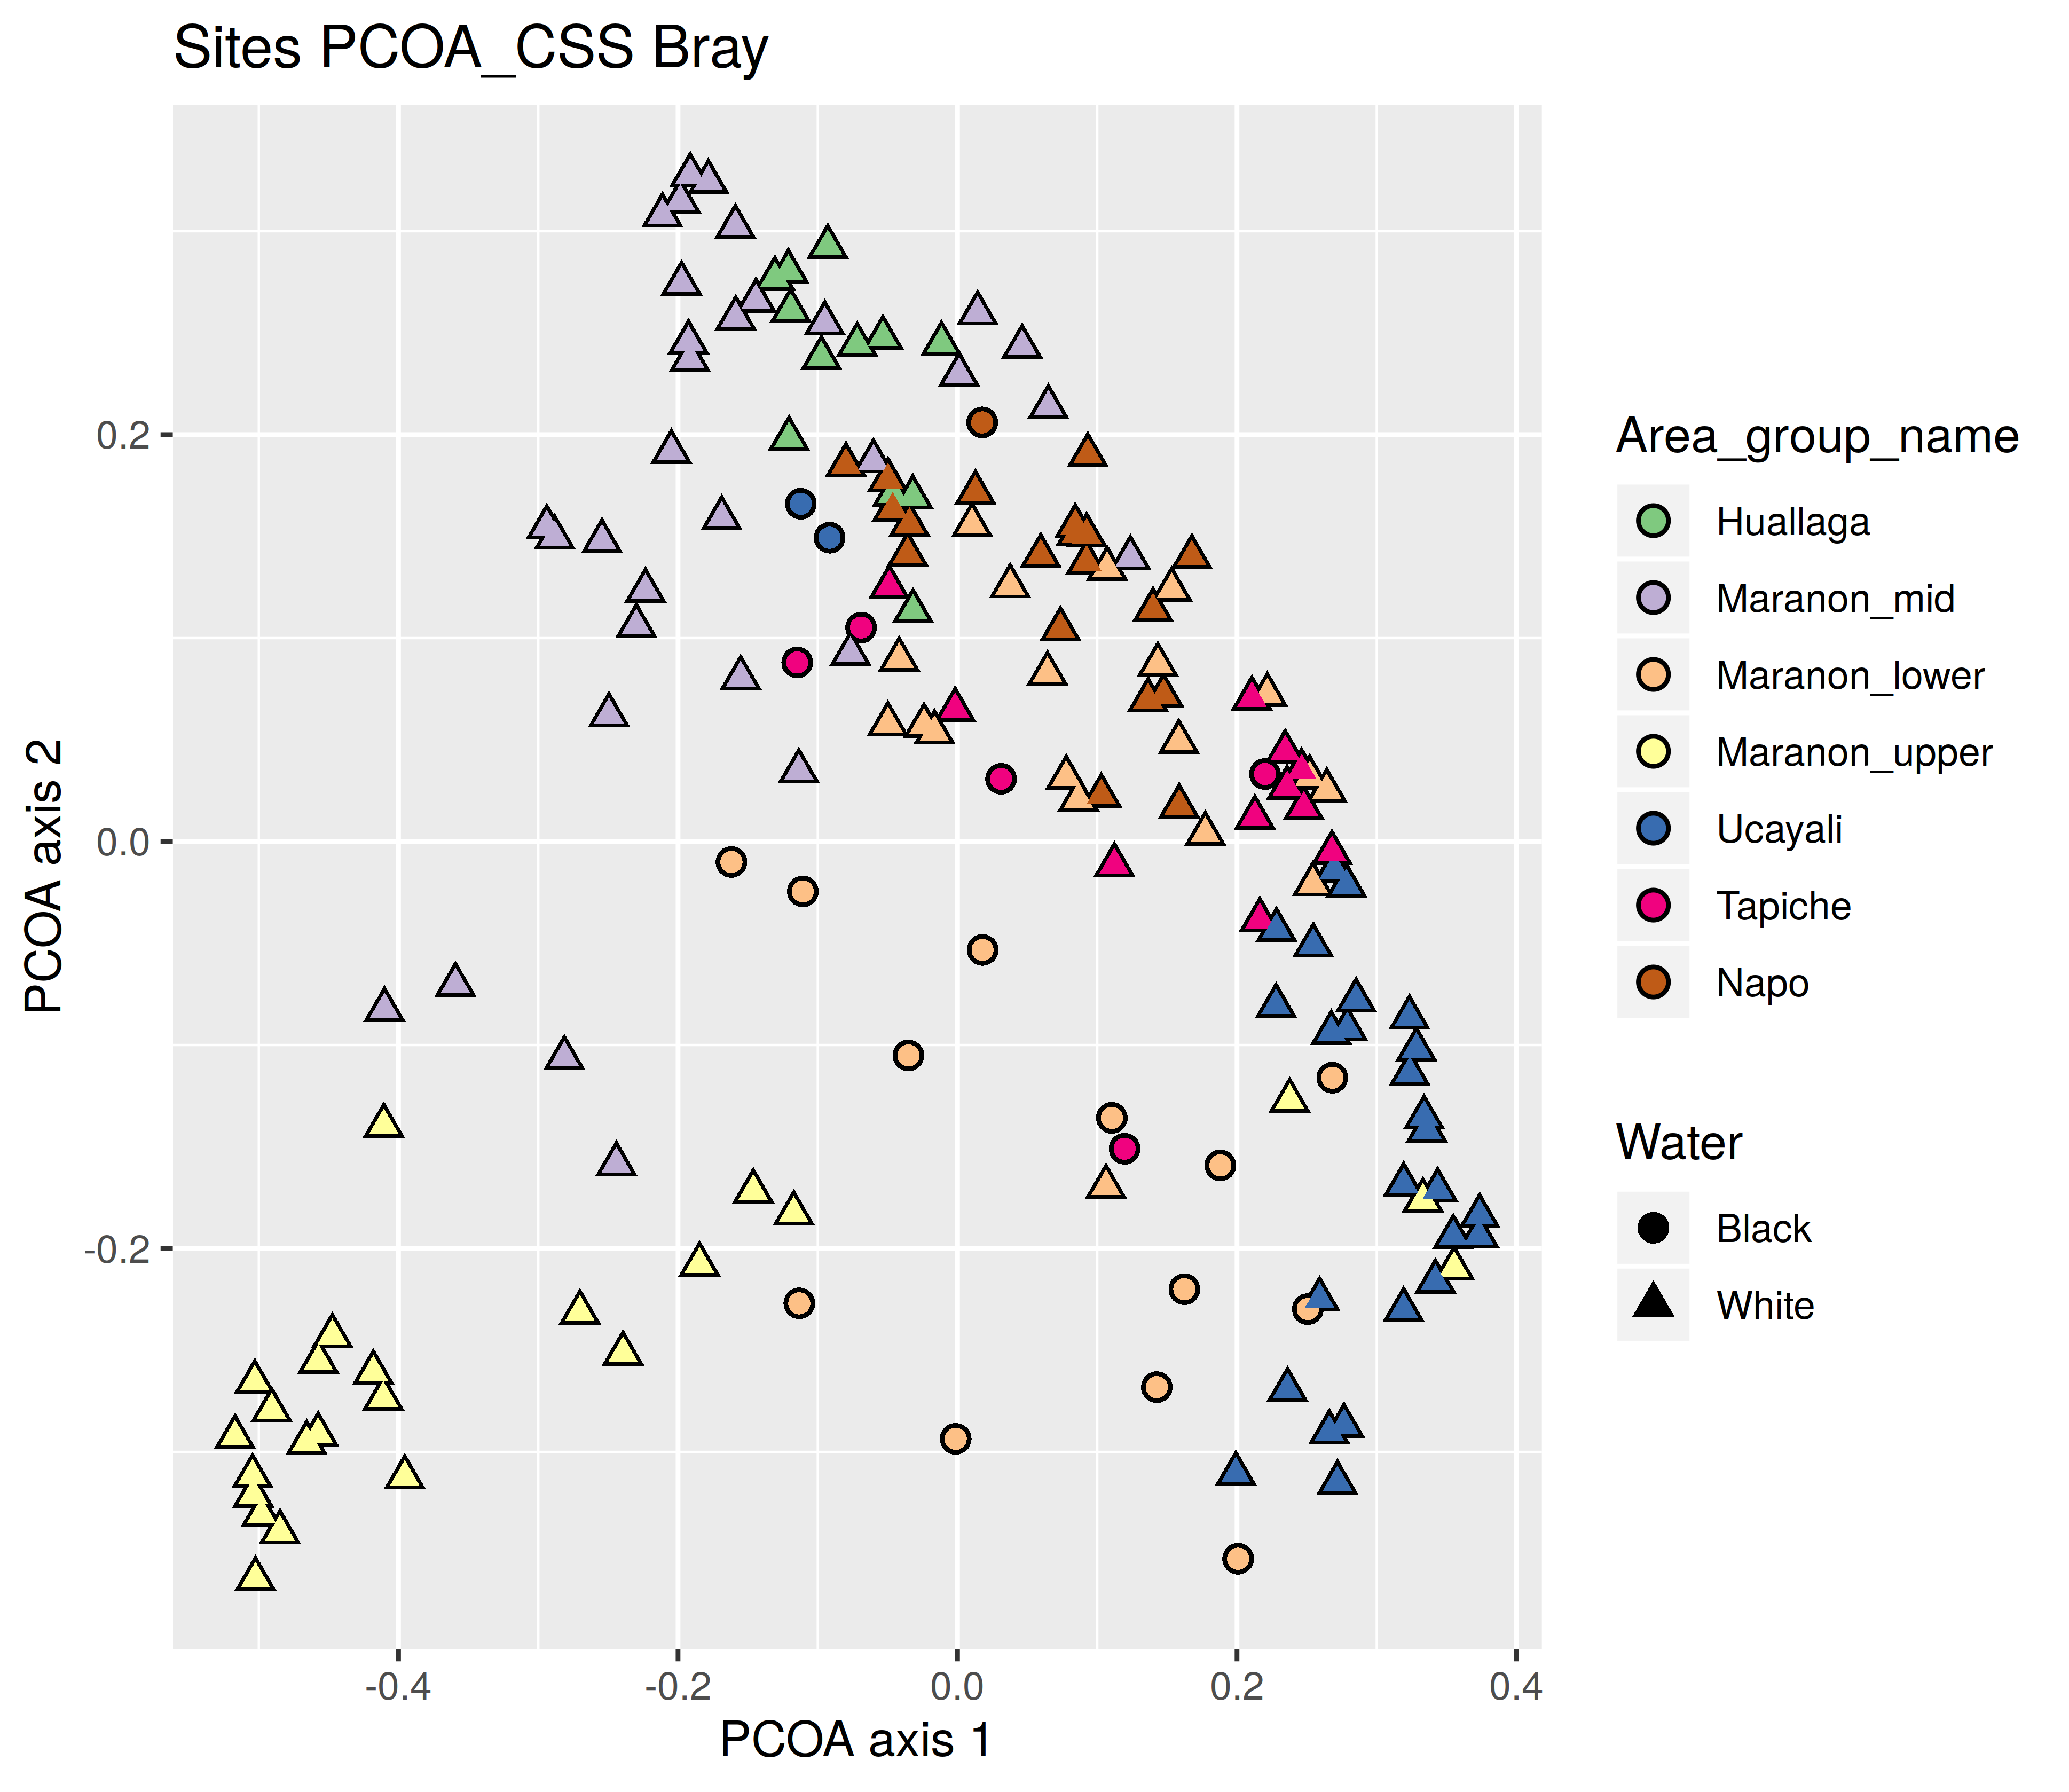
\includegraphics[width = \textwidth]{pcoa12otucss}
		\caption{}
		\label{fig:pcoa12otucss}
	\end{subfigure}
	\caption{Ordination plots for the CSS normalised data. \ref{fig:nmds12otucss} shows an NMDS plot of the data and \ref{fig:pcoa12otucss} a PCoA using Bray-Curtis measure. Both methods separate white and black water samples better than their respective ordination methods applied to non-normalised data.}
\end{figure}

We will be checking if this normalisation method and transformation produces any significant improvements (over the unnormalised dataset) in the classifiers ability to determine the river colour. 

%%Normalization, which is the process where systematic variability is identified and removed, is therefore a vital part of the data analysis. 
%https://www.ncbi.nlm.nih.gov/pmc/articles/PMC5910605/
% A substantial part of this variability is systematic and affects multiple genes and/or samples in a similar way. One example of systematic variability is the differences in sequence depth, where each sample is represented by a varying number of reads [13]. Systematic variability also comes from other technical sources, such as inconsistencies in the DNA extraction and sample handling, varying quality between sequencing runs, errors in the read mapping, and incompleteness of the reference databasescd 


\subsection{Feature Correlation}

A big minority of OTUs in our data set have been found to have an absolute Spearman correlation of more than 0.9 with at least one other OTU. This correlation has a biological underpinning as it is expected that the abundance of species in a river environment would co-vary along it's length. Relationships between species in an environment have been modelled and can take many forms, like parasitic (the abundance of OTU1 and OTU2 is increased and decreased and they are both present), competitive (the abundance of both OTU1 and OTU2 is decreased when they are both present), and mutual (the abundance of both OTU1 and OTU2 is increased when they are both present). More complicated, non-linear correlation networks exist in nature between more than two species that are very difficult to capture even with large amounts of unbiased data \cite{weiss_correlation_2016}. 



For our problem at hand, recovering such correlation networks is not of interest. We are more interested in selecting the best features from our data that would aid in the classification. Thus, we used the Spearman correlation with a threshold of 0.9 to remove 122 OTUs to create a new data set without highly correlated OTUs. 










%%~~~~~~~~~~~~~~~~~~~~~~~~~~~~~~~~~~~~~~~~~~~~~~~~~~~~~~~~~~~~~~~~~
%% DATA SPLITTING
%%~~~~~~~~~~~~~~~~~~~~~~~~~~~~~~~~~~~~~~~~~~~~~~~~~~~~~~~~~~~~~~~~~
\section{Splitting}
\label{sec:splitting}

Together with the OTU table, our data also include the location of the samples in the rivers (in Easting and Northing coordinates) and in which part of the river they belong to. Because of this location attribute, our samples cannot be said to be independent. Thus, the way we choose to split our data into training and testing sets will surely affect the accuracy of the classifier. For example, testing on a set that is composed of samples maximally distant from the ones in the training set (see Figure \ref{fig:groupsamp}) will produce different results than testing on a set with all samples in close proximity to the ones in the training set (see Figure \ref{fig:stratsampl}).

To avoid choosing a split method, several ones have been employed that represented different splitting conditions. The classifiers have then been tested on all of them so as to evaluate how well they can perform under various circumstances.
%% Stratified an group folds for tain test split plot
\begin{figure}[h]
\centering
\begin{subfigure}{0.4\textwidth}
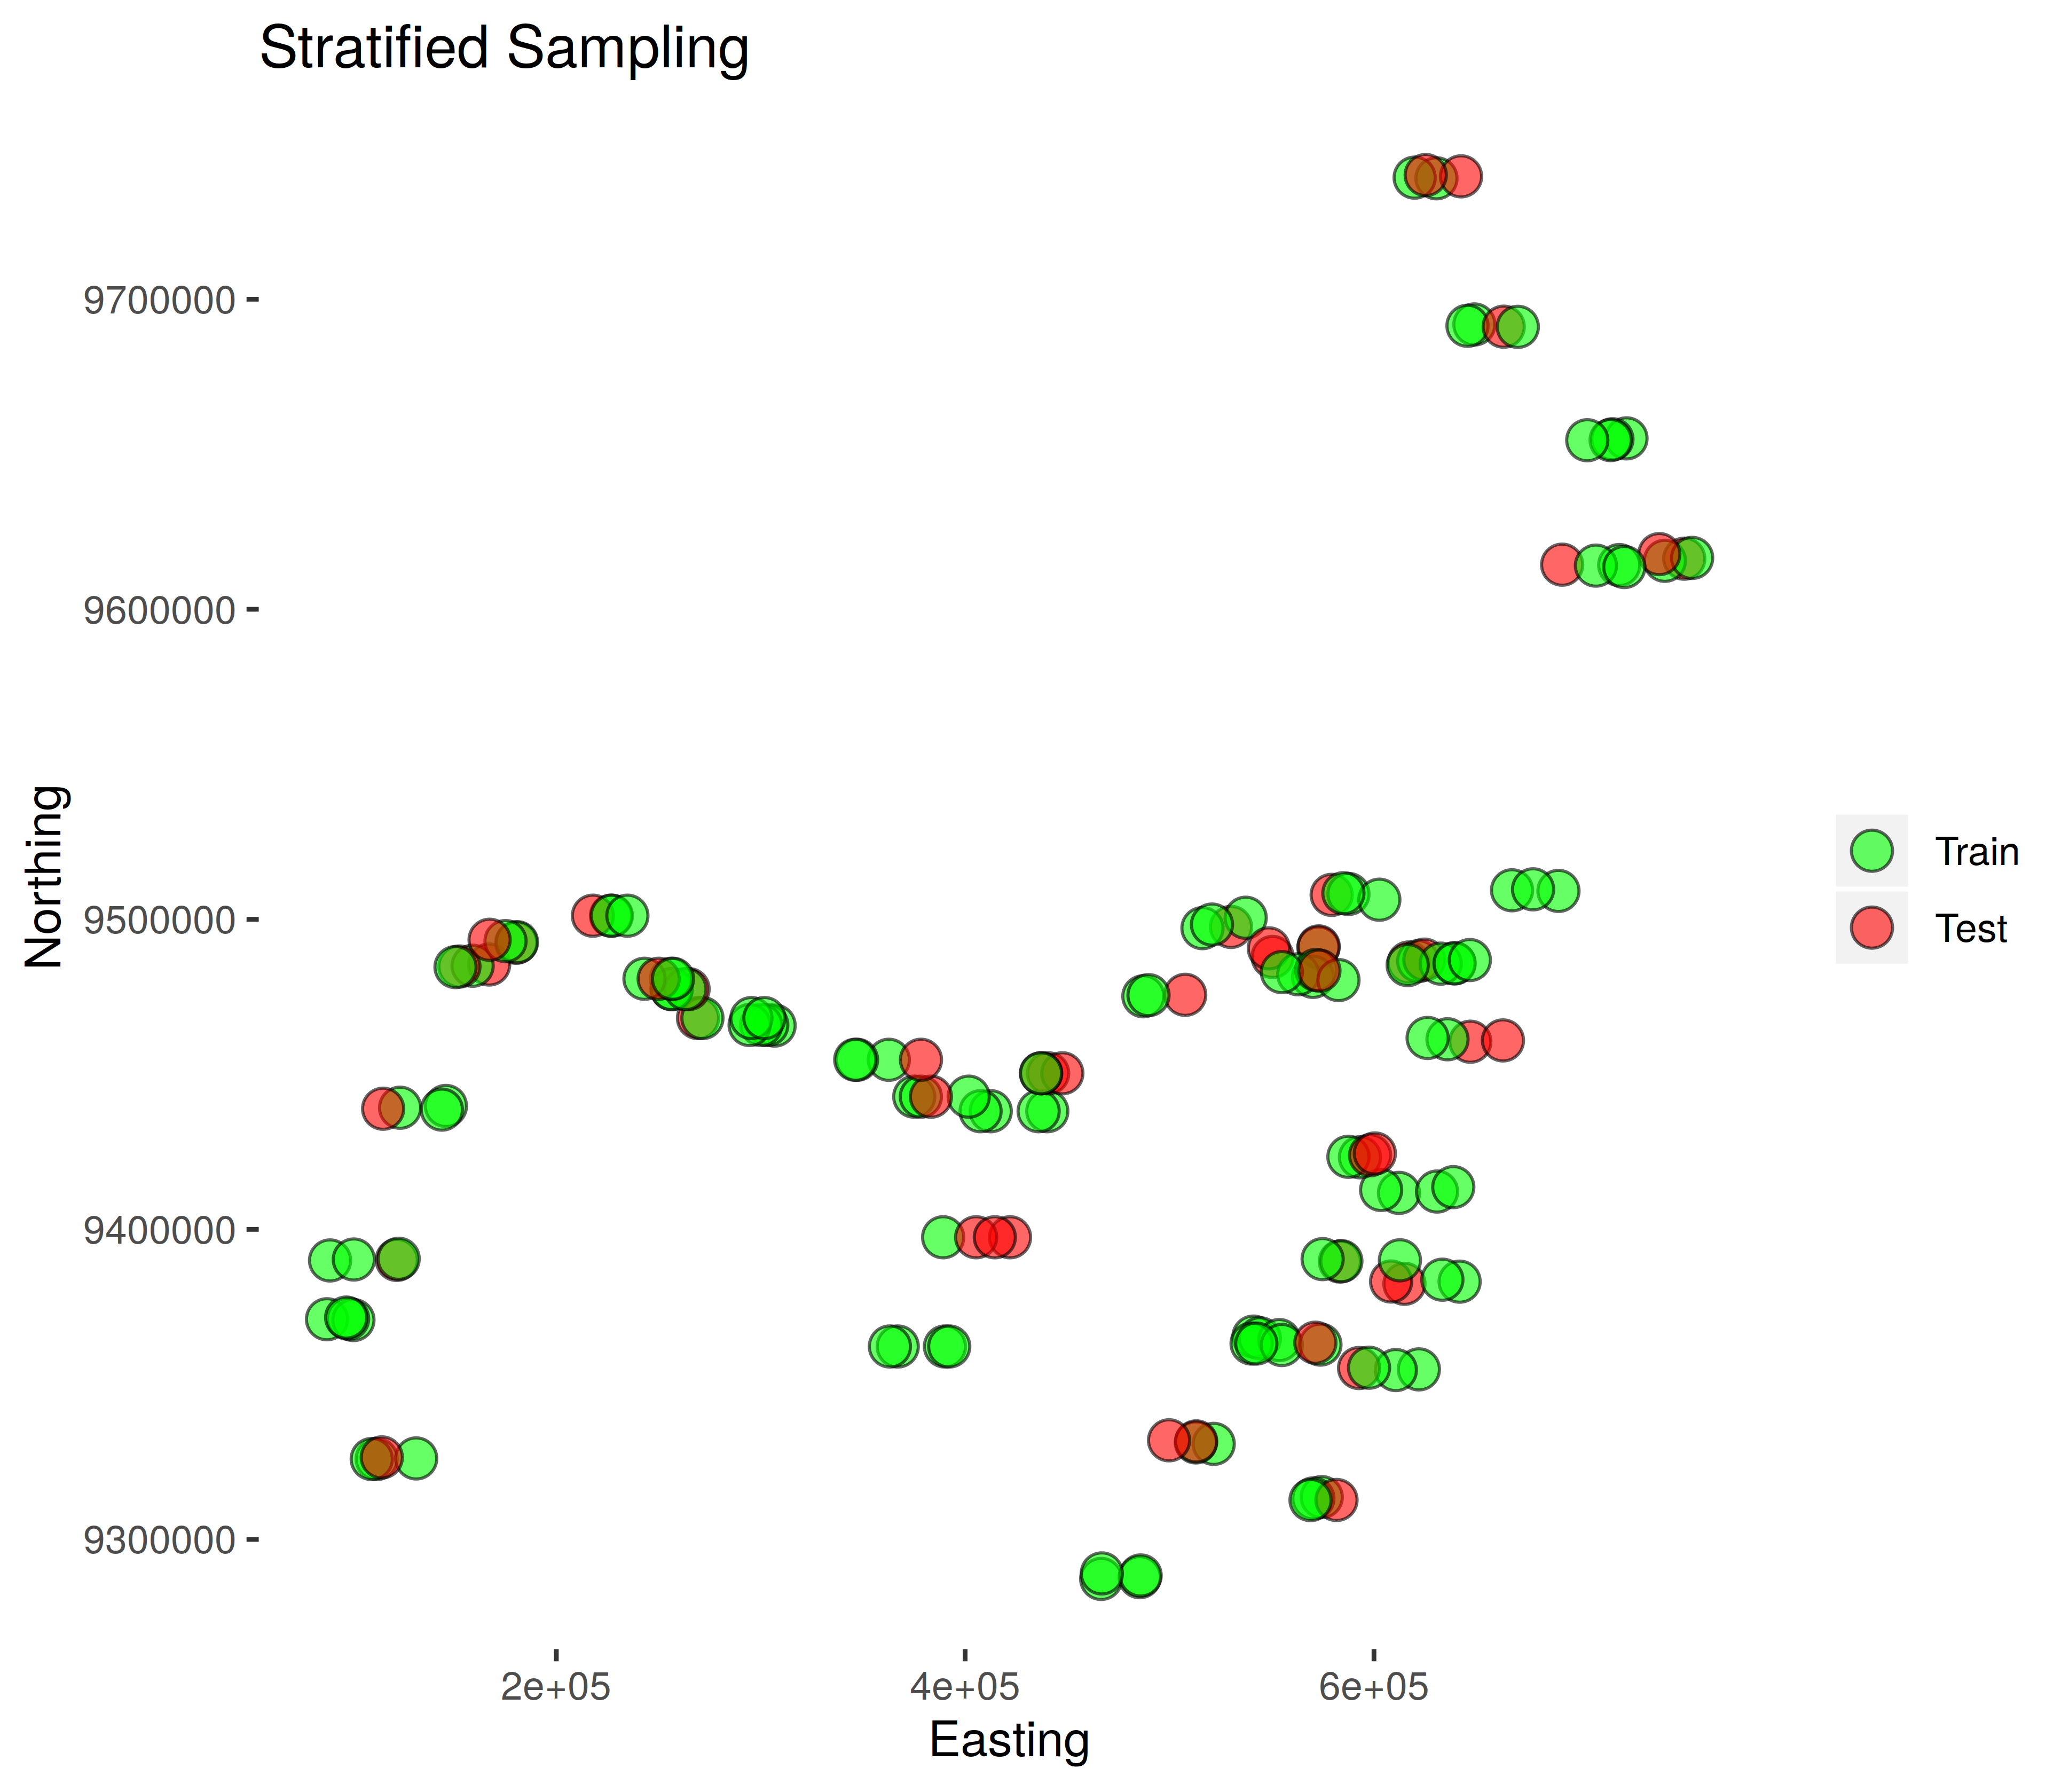
\includegraphics[width = \textwidth]{stratsamp.png}
\end{subfigure}
\begin{subfigure}{0.4\textwidth}
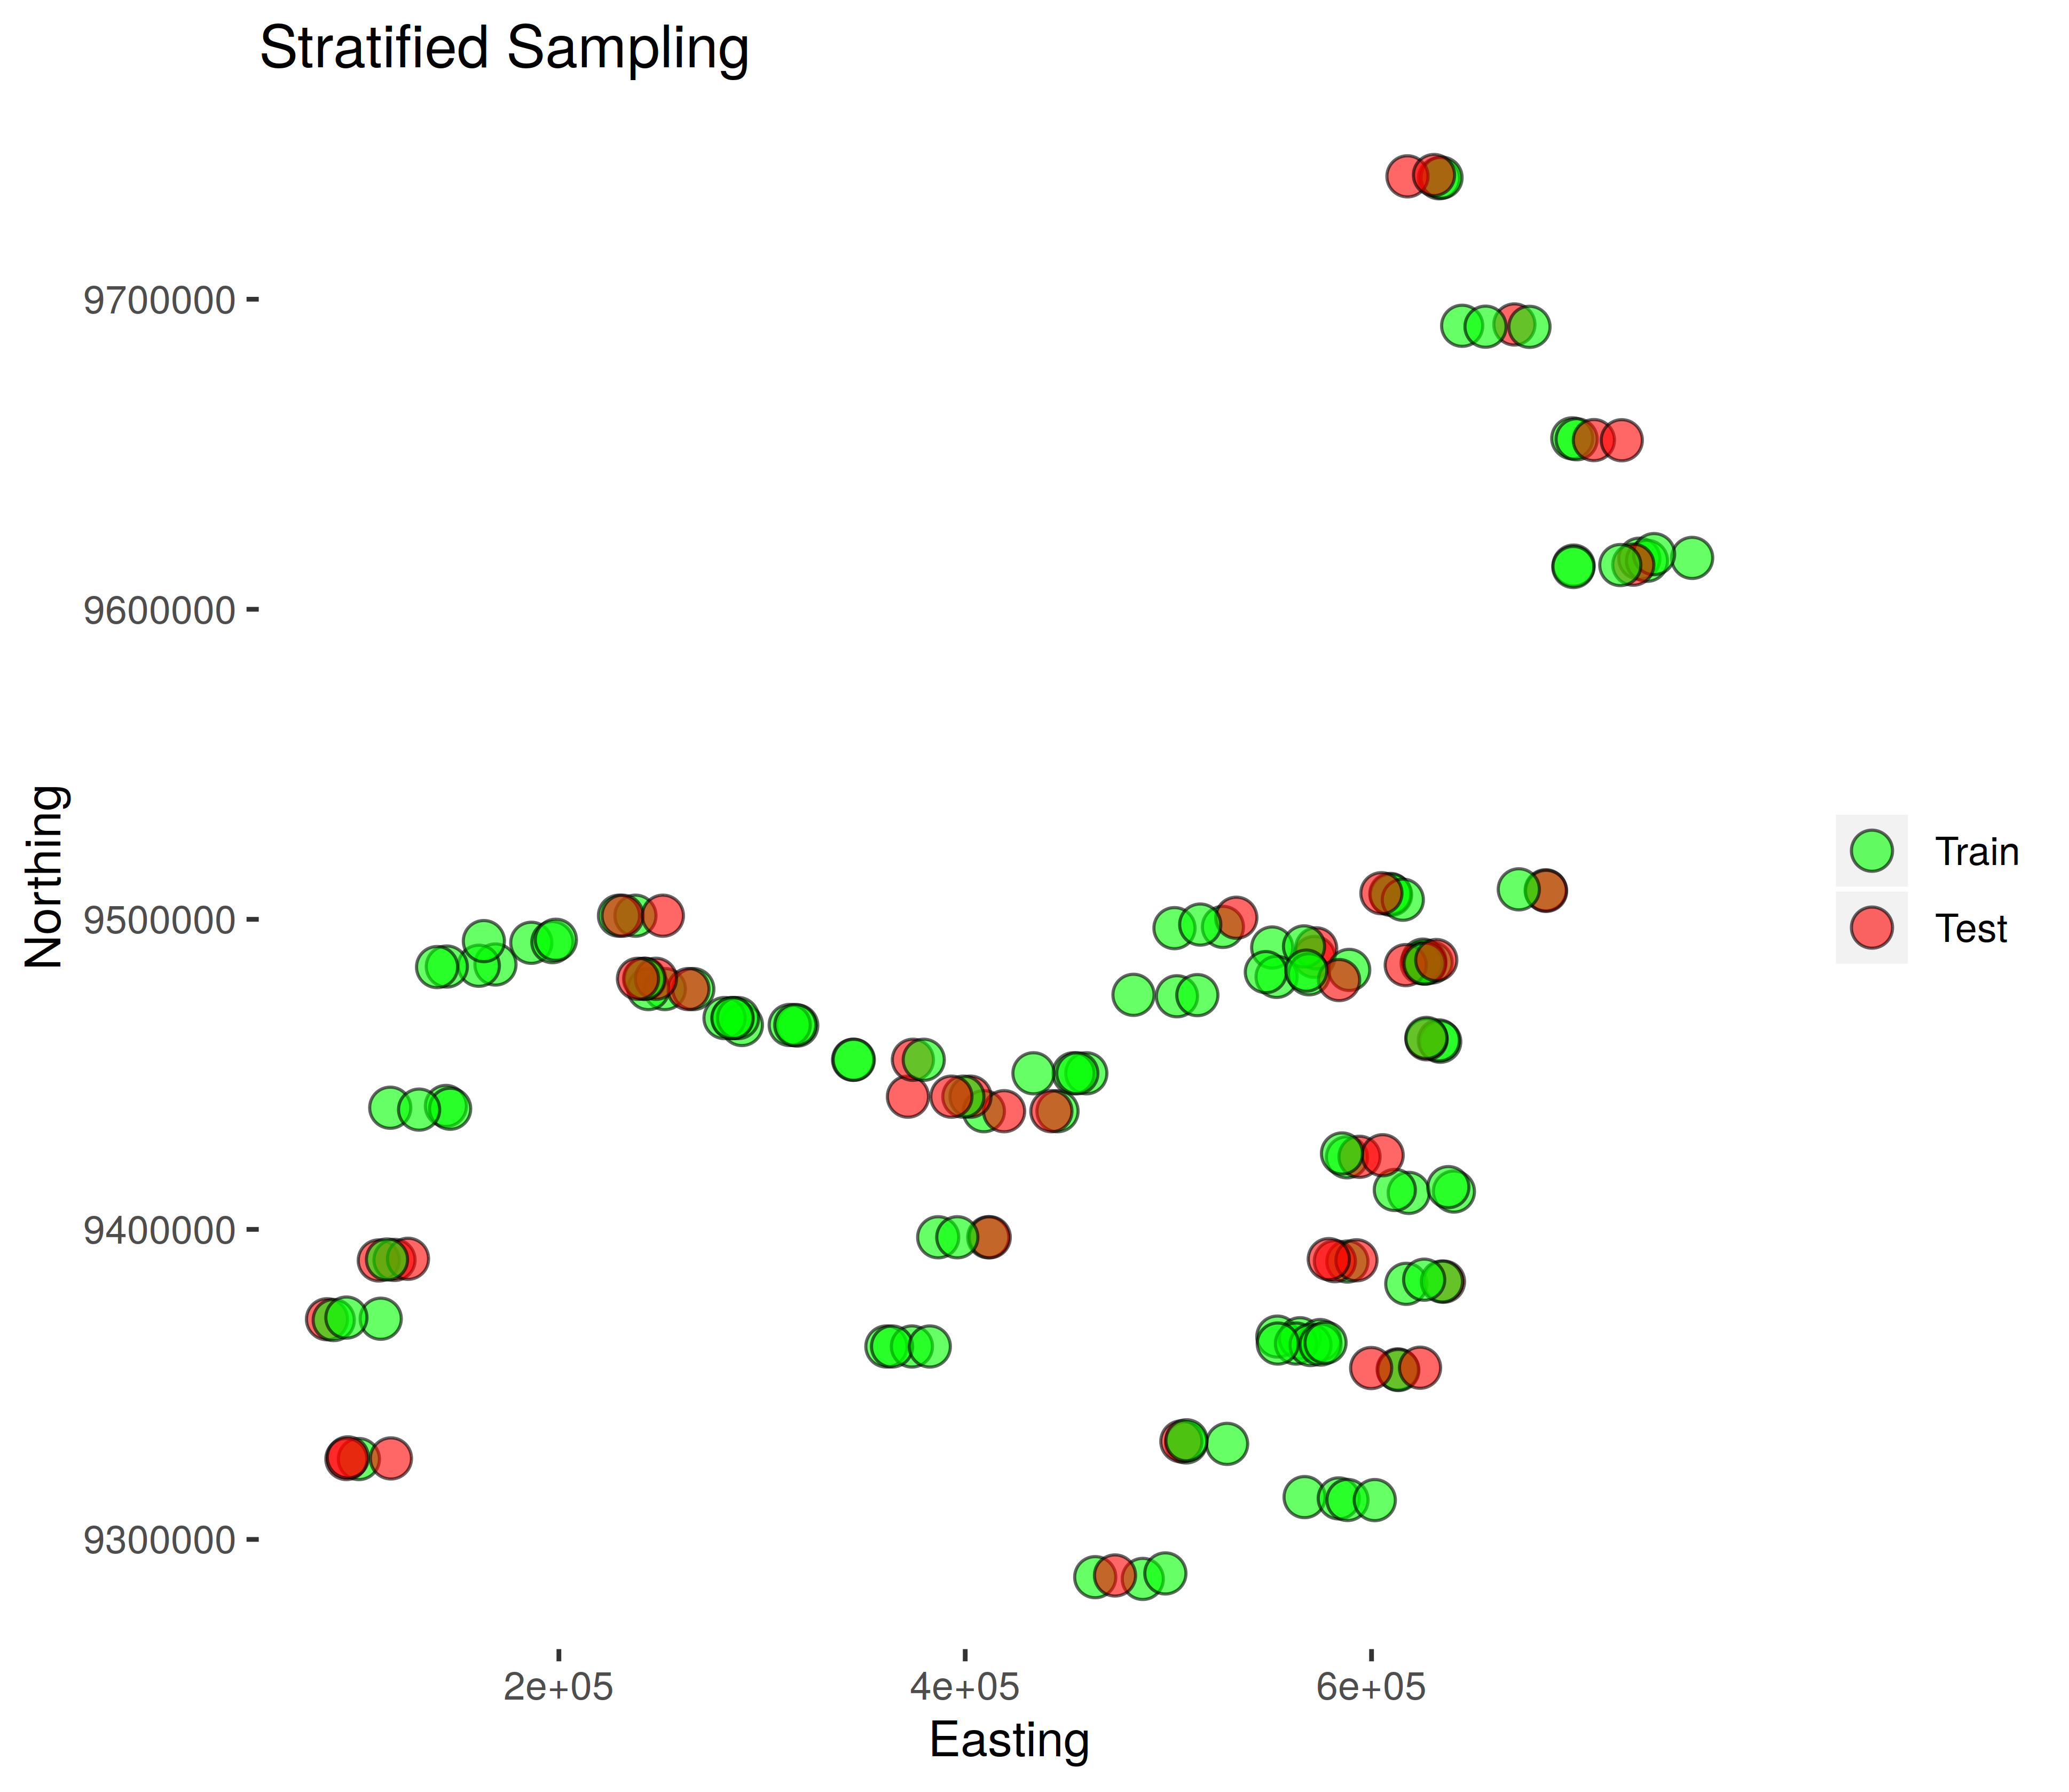
\includegraphics[width = \textwidth]{stratsamp2.png}
\end{subfigure}
\caption{Test set samples are geographically among Train set samples. This represents a maximally similar split which is created by ensuring constant distribution of samples in each part of the river in both the Train and Test set.}
\label{fig:stratsampl}
\end{figure}

%Group sample plot
\begin{figure}[h]
\centering
\begin{subfigure}{0.4\textwidth}
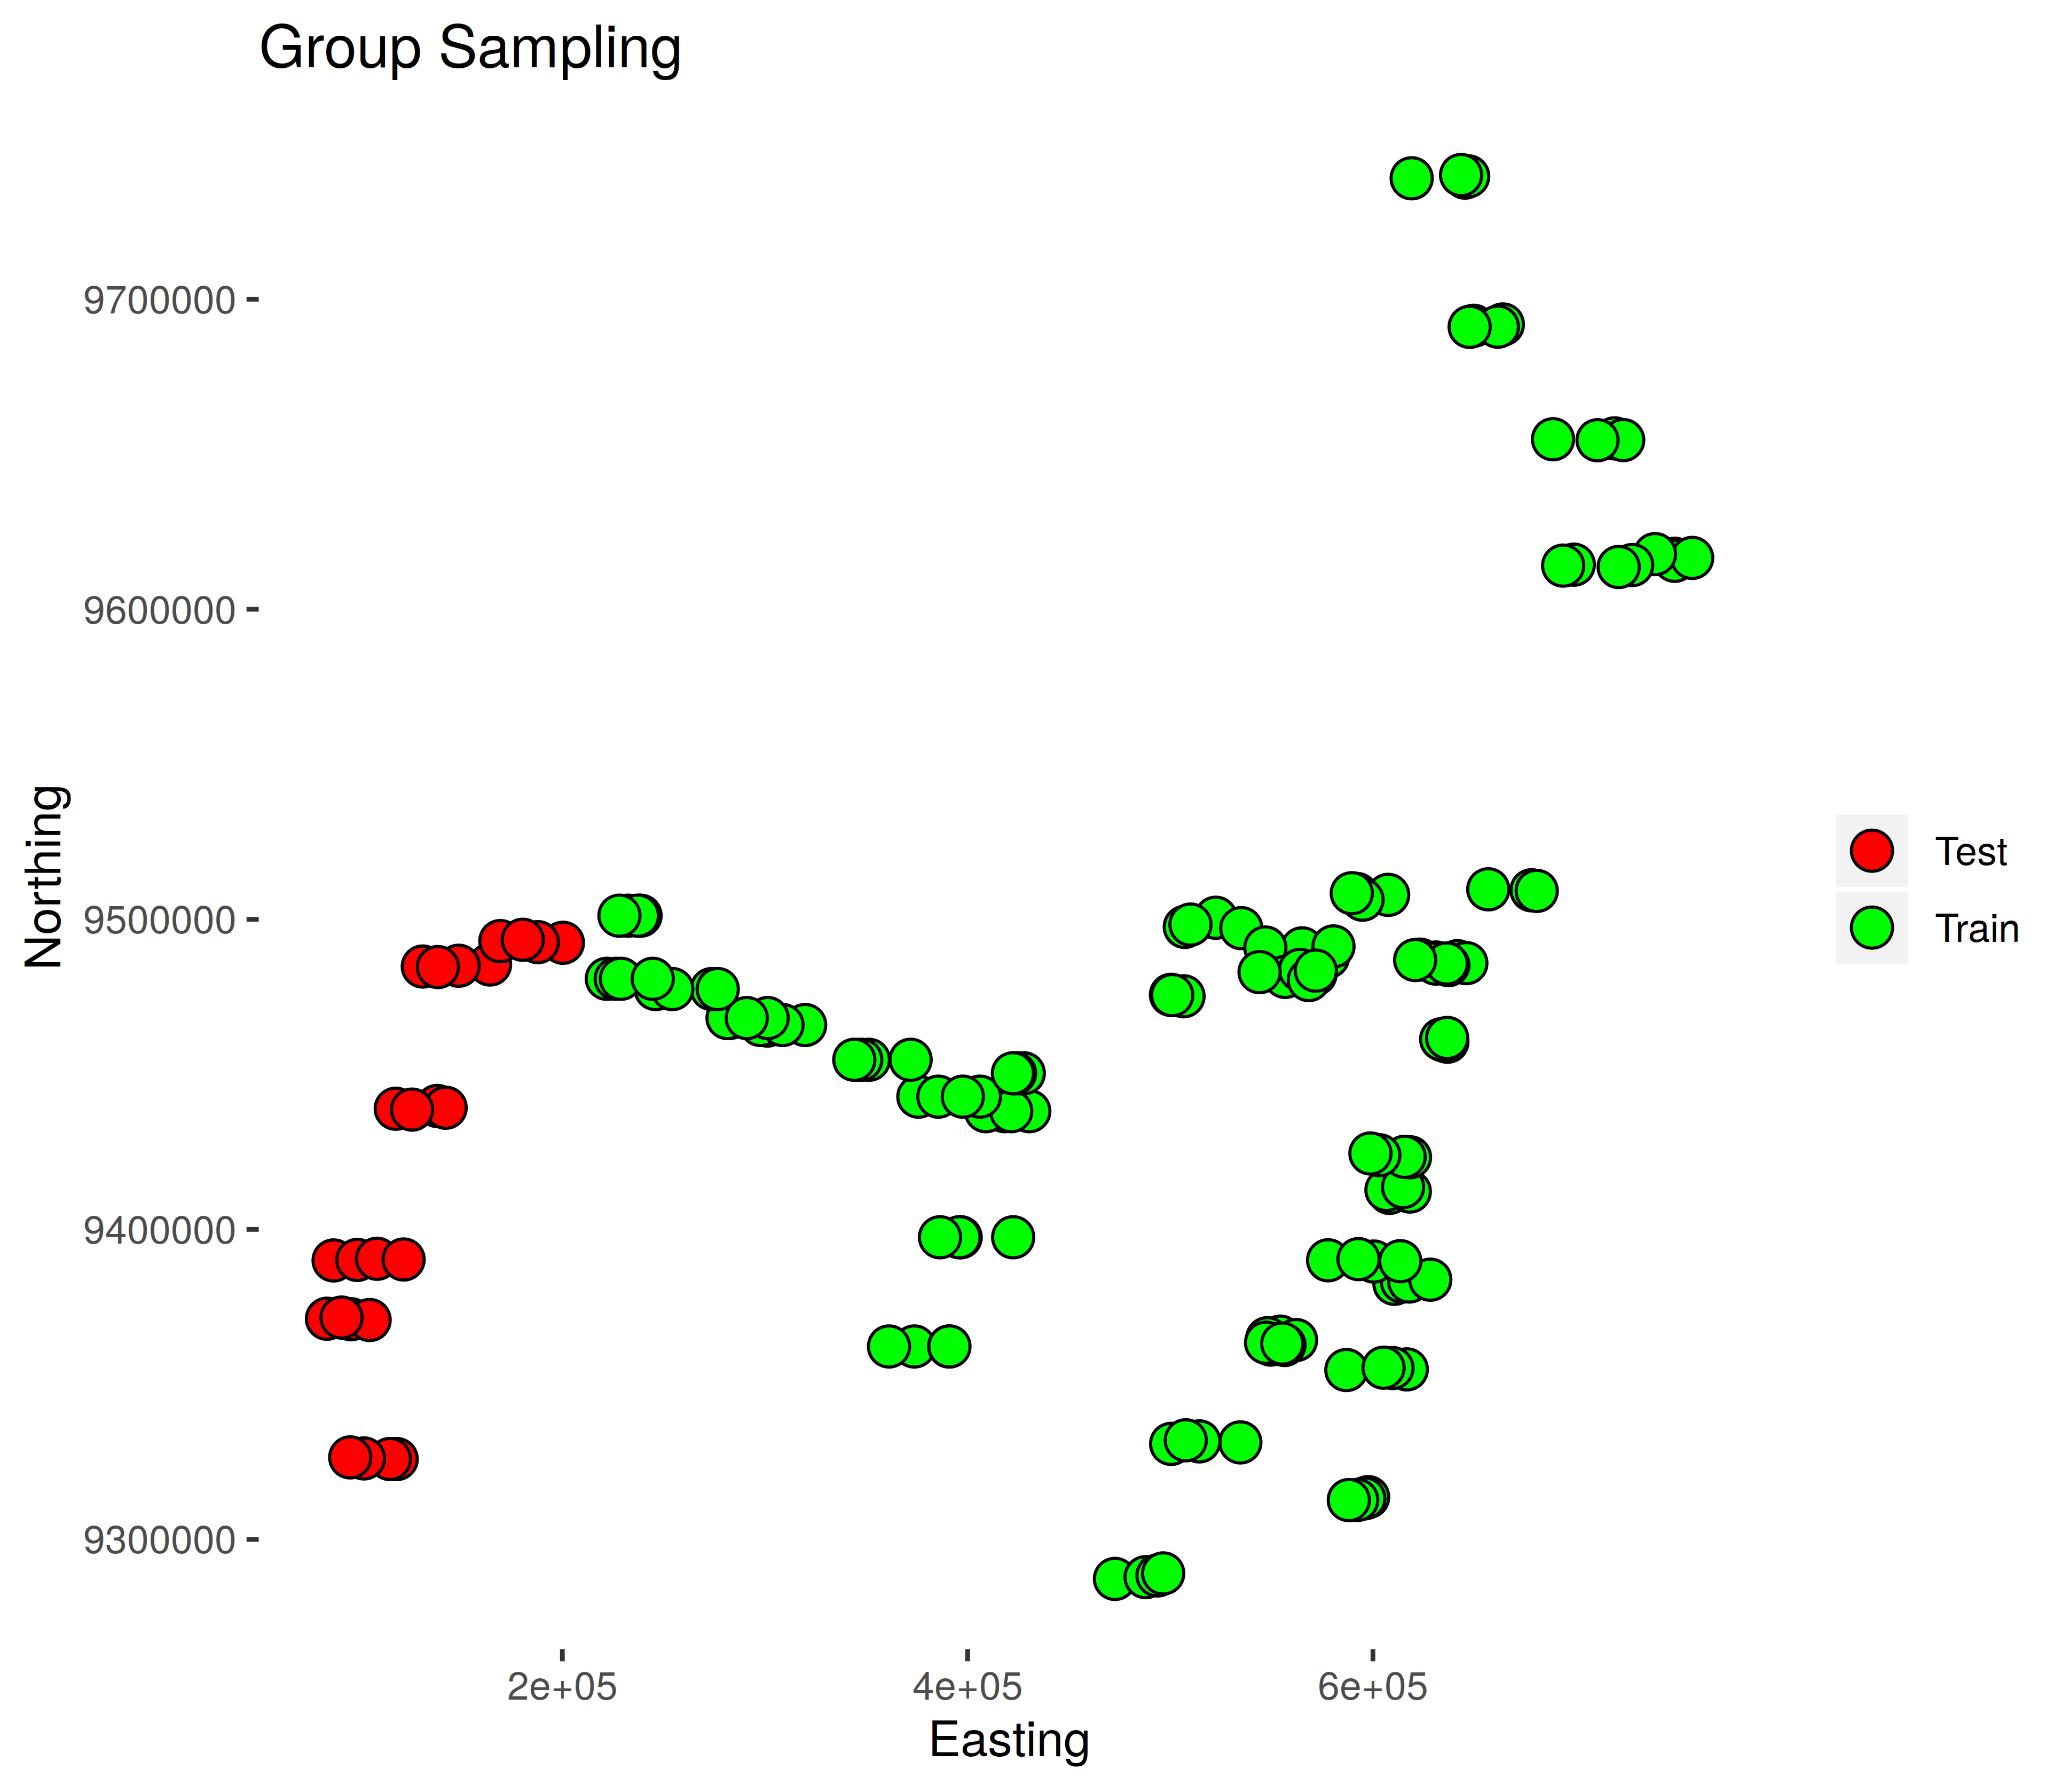
\includegraphics[width = \textwidth]{groupsamp.png}
\end{subfigure}
\begin{subfigure}{0.4\textwidth}
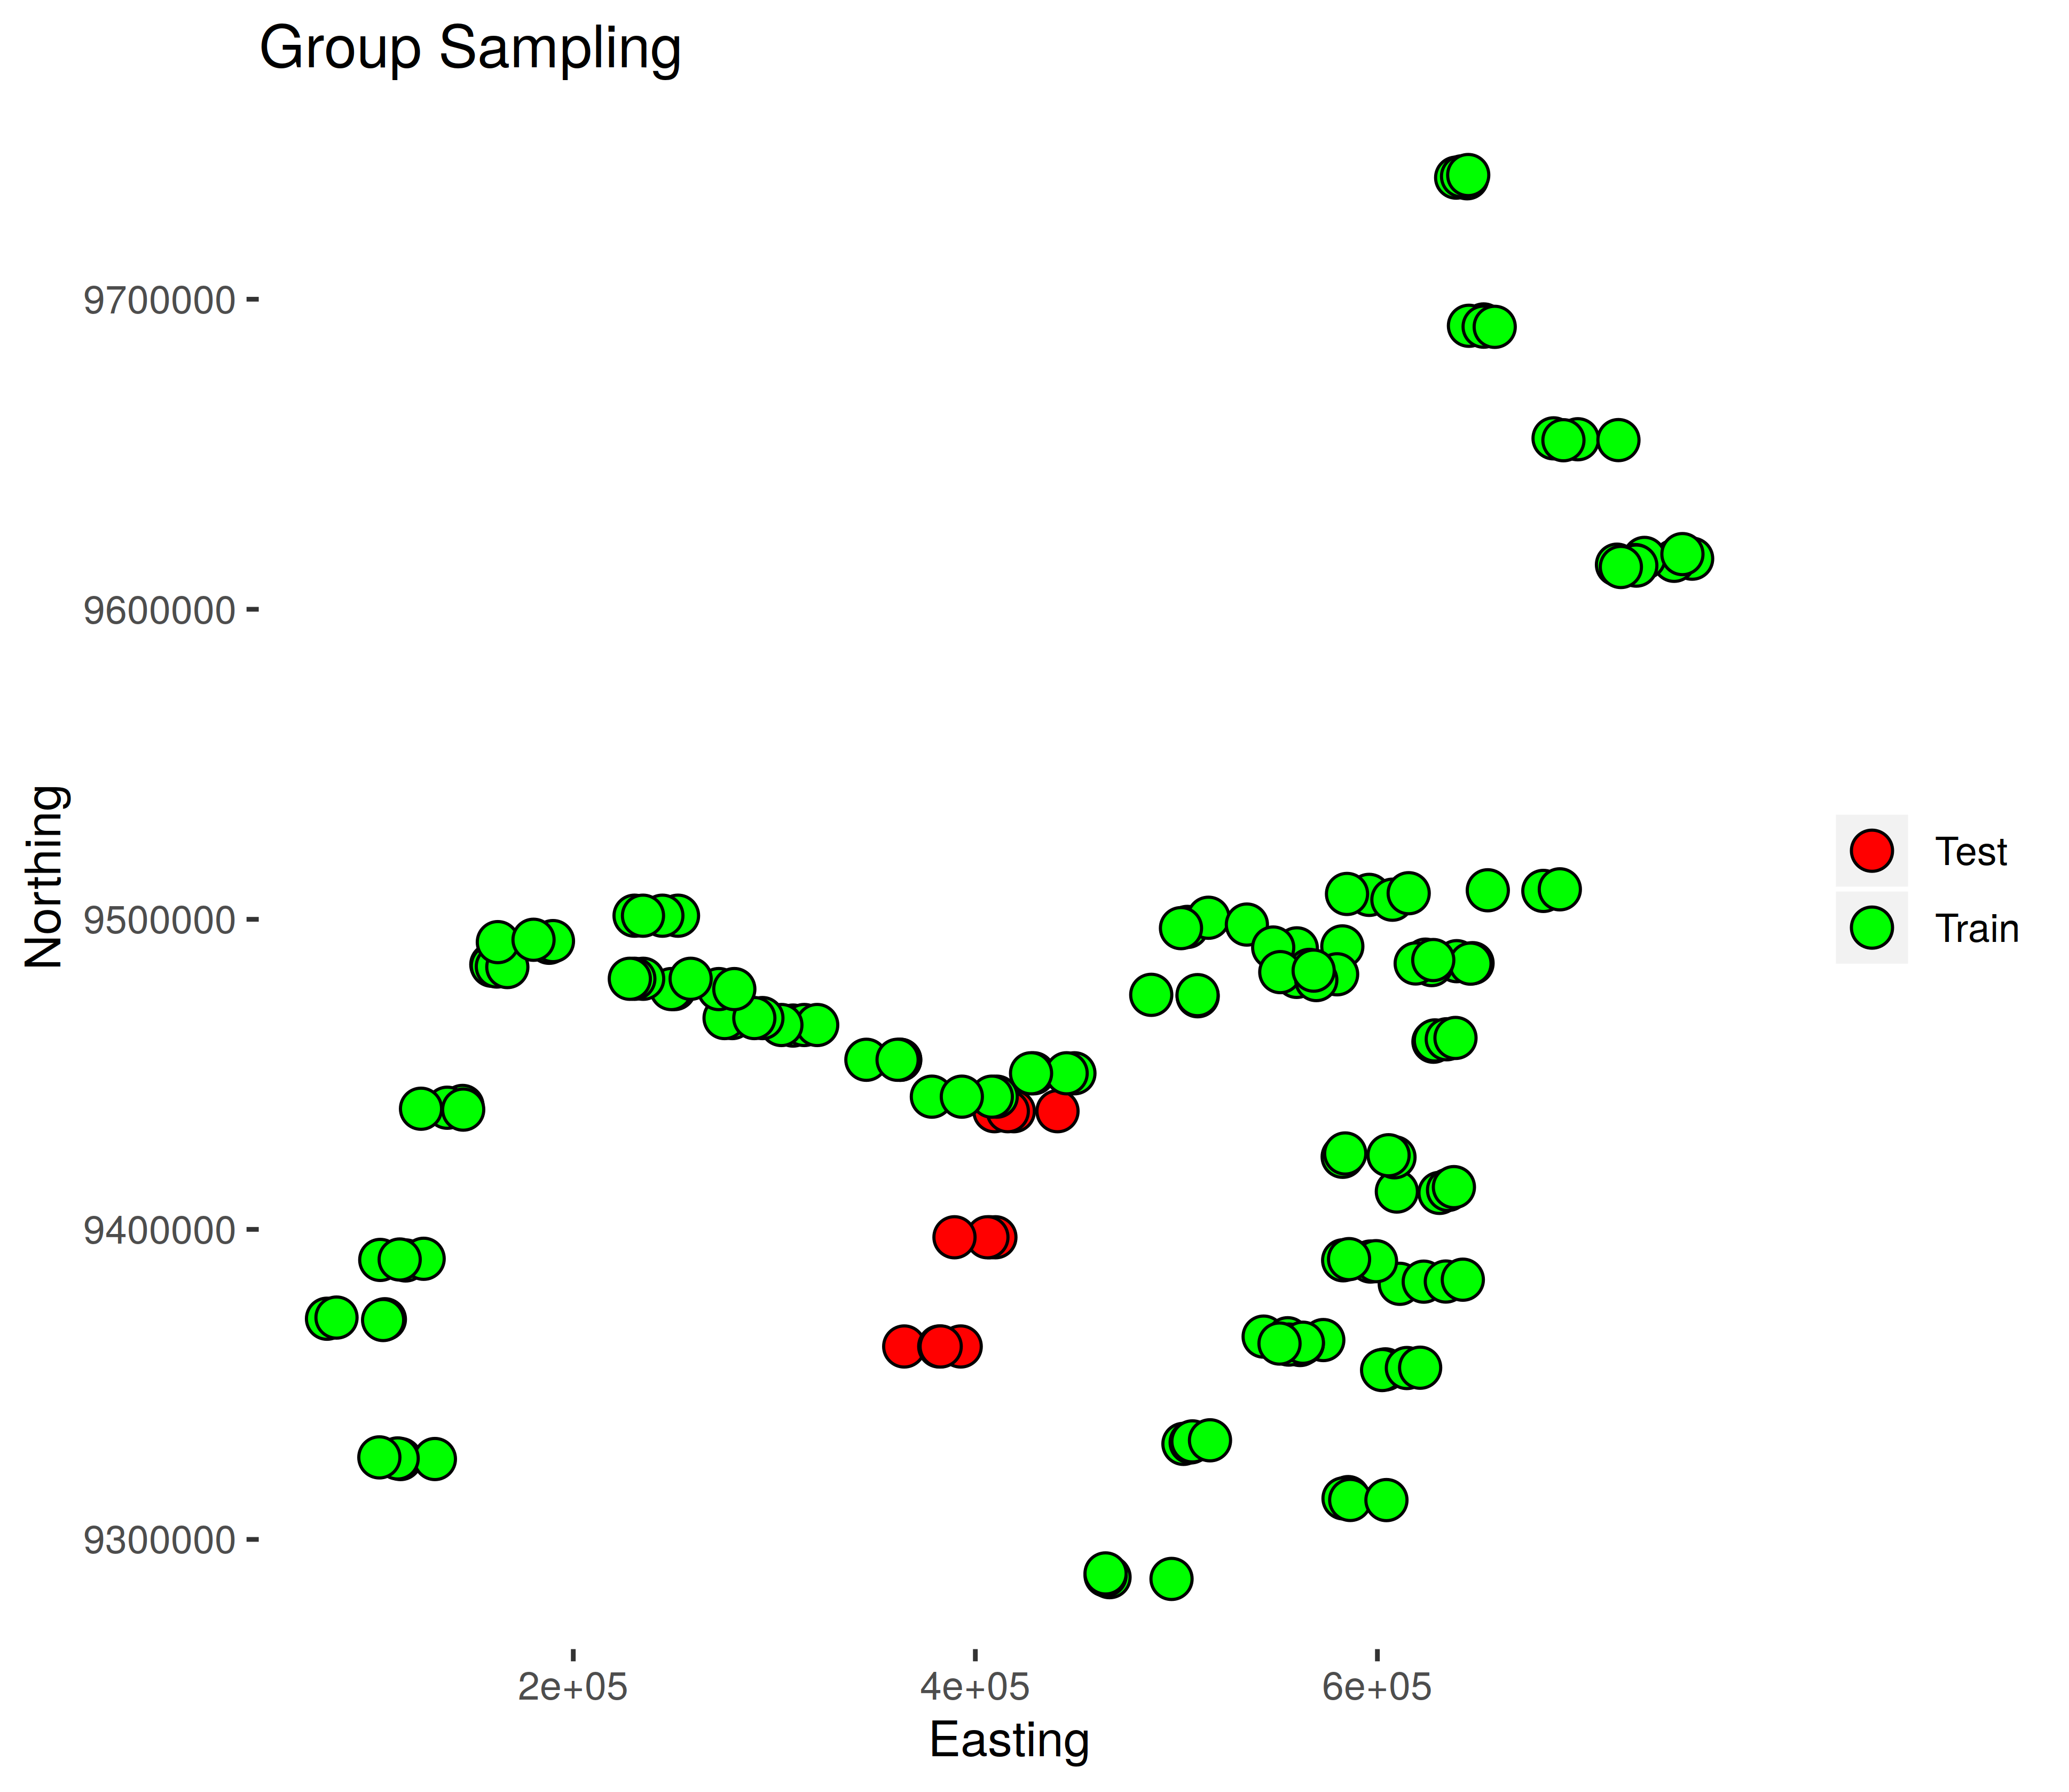
\includegraphics[width = \textwidth]{groupsamp2.png}
\end{subfigure}
\caption{Test set samples are geographically distinct from Train set samples. This represents a maximally dissimilar split which is created by choosing a different part of the river as the Testing set.}
\label{fig:groupsamp}
\end{figure}




%Validation sets
In addition to splitting the data into training and test sets, the train set was further split into validation sets so as to tune the hyperparameters of the models. The splitting into validation sets followed the same principle/method as the train-test split. So if, for example, the train and test sets were split using the maximally similar approach, the validation sets produced from the train set were chosen so as to be maximally similar to the remaining set.


The steps of testing a classifier using a specific split method are as follows:
\begin{enumerate}
\item The data set is split into train and test sets based on the splitting method of choice. 
\item The train set is split into $K$-folds using the same method for the train-test split.
\item A set of hyperparameters and potential values are chosen for the cross-validation procedure. For example, in Logistic Regression a set of numbers ranging from 0.001 to 20 is chosen for the sparsity parameter and the set $\{True,False\}$ is chosen for the intercept parameter    
\item The classifier is trained on the $K-1$ folds and tested on the remaining validation set for all possible combinations of hyperparameters (e.g. the Logistic Regressor is trained with hyperparameters $\{0.001,True\},\{0.001,False\},\{1.001,True\},\{1.001,False\}$ etc...).
\item Step 4 is repeated for all the $K$-folds (by training on the $K-1$ and testing on the one left out). The average score across the validation sets is found for each hyperparameter combination and the classifier is retrained on the train set using the best hyperparameters set.
\item The retrained model is tested on the test set and the confusion matrix is calculated.
\item Steps  1 through 6 are repeated a number of times for different train-test splits using the same split principles. The confusion matrix for each repetition is stored and added at the end of the process.  
\end{enumerate}

 
The best hyperparameters are the ones that maximise either the F score or accuracy. The former combines both the precision and recall of the validation test. Precision is the number of correctly identified positive results divided by the number of all positive results returned by the classifier. Recall is the number of correctly identified positive results divided by the true number of positive results. The score is the harmonic mean of the two
\begin{equation}
	F_1 = \frac{2}{\text{recall}^{-1} + \text{precision}^{-1}}.
\end{equation} 
If black water was chosen as the positive result then there would be cases that recall would be undefined. This is because in the case of maximum dissimilarity, a validation set might end up with only white water samples (thus only negatives). So recall, which measures how many positive observations were correctly identified from the total number of positive observations, would be $\frac{0}{0}$. Thus, white samples were chosen as the positive observations.

The whole testing procedure was repeated using accuracy as the metric for picking the best hyperparameters. This is because the F score might lead to choosing classifiers that minimise False Negatives (maximising recall). 

This procedure can be repeated for different features (data sets), so as to evaluate how feature selection and transformations can alter the results.
% The best classifier for the particular features and splitting method is the one which has the highest mean score across all train-test splits. 
 The various data sets used to test the classifiers on are summarised in table \ref{table:features}.
\begin{table}
	\caption{Features used in Classification}
	\centering
	\label{table:features}
	\begin{tabularx}{\textwidth}{l X  }
		\hline 
		Features used &Description of dataset\\ 
		
		\hline
		OTU &The OTU table as it is without any modifications done to it \\
		OTU LOW & The OTU table without highly correlated features\\
		OTU CSS & The normalised OTU table using CSS\\
		OTU Min CSS & The normalised OTU table using CSS without samples with total counts of less than 10000 reads  \\
		OTU CSS LOG & A $\log_2$ transformed OTU CSS \\
		PCoA Bray-Curtis &The transformation of the OTU table with PCoA using the Bray-Curtis measure  \\
		PCoA Bray-Curtis CSS &The transformation of the normalised OTU table with PCoA using the Bray-Curtis measure\\
		
		\hline 
	\end{tabularx}
\end{table}


The baseline performance for this problem was also devised so that meaningful evaluations could be made of the classifiers. This method is essentially setting the `coin flip'/naive rate; prediction based on prior probabilities of the classes. Using their distribution on the whole data (87.2\%) set would be an unfair baseline for the classifiers since they are trained on a fraction of it, and the proportions of black and white water samples change significantly with the train set. 

Thus, for every train-test split we calculated the prior probability $P(C=1)$ of a sample being white using the train set by dividing the number of white samples to the total number of samples. Then, for each observation in the test set $y_i$ we calculated the expected times the `coin' would identify it correctly and falsely
\begin{align}
	E(\text{Correct Prediction}|y_i ) = y_i*P(C=1) + (1-y_i)*(1-P(C=1)) \\
	E(\text{False Prediction}|y_i) = (1-y_i)*P(C=1) + y_i*(1-P(C=1)).
\end{align}
Then a confusion matrix was constructed (see table \ref{table:baseline}) using the total number of white $N_{white}$ and black $N_{black}$ water samples in the test set.
\begin{table}[h]

	\centering

	\begin{tabularx}{\textwidth}{l| c c}
	 
		 &Predicted Black&Predicted White\\ 
		
		\hline
		Actual Black&$N_{black}*E(\text{Correct}|\text{Black} )$&$N_{black}*E(\text{False}|\text{Black})$\\
		Actual White& $N_{white}*E(\text{Correct}|\text{White} )$&$N_{white}*E(\text{False}|\text{White})$

	\end{tabularx}
	\caption{Confusion matrix of baseline benchmark}
		\label{table:baseline}
\end{table}

{ \large\bf Maximising Similarity} \\
\textit{Aim}: Evaluate how well the classifiers perform when they are tested on a set which is similar geographically to the train set.\\
\textit{Method}: Testing and validation sets are made up of samples coming from every part of the river. Care is taken to ensure that no geographical area is over represented. This is done using Stratified sampling (using the method StratifieKfold) where the strata (or groups) are the areas of the rivers the samples belong to. Stratified sampling ensures that the distribution of test or validation samples in each area is approximately the same as for train samples.




{ \large \bf Maximising Dissimilarity}\\
\textit{Aim}: Evaluate how well the classifiers perform when they are tested on a set which is dissimilar (or far away) geographically to the train set.\\
\textit{Method}: Testing and Validation sets are made up of all the samples which belong to a particular area of the river. For example, the test set might be constituted by all the samples in the Upper Marañón area, and the validation sets by all the remaining areas (Huallaga, Min Maranon, Lower Maranon, Ucayali, Tapiche, Napo). The method used to produce these splits is called GroupKfold.

{\large \bf Random Splits}\\
\textit{Aim}: Evaluate the performance of the classifiers on train and test sets obtained by random splitting
\textit{Method}: Test and Validation sets are obtained by randomly splitting the data. Care is taken to ensure that the balance of white and black water samples is the same across splits. This is done using Stratified sampling with the colour of the river as the strata.


{ \bf Ideal Splits}
An ideal sampling method would take into account the spatial correlation structures between the samples, besides just their location. Since the river flows eastwards from Maranon Upper down to all other streams, samples collected upstream would inevitably affect those from downstream, but the opposite might not be true. Thus, euclidean proximity of the river samples is not always a good enough indicator for detecting similarity between samples. For example, sample A collected near the opening of the Tapiche stream and sample B collected a bit further South of the opening, in the Ucayali stream, will have a smaller distance between them than with other samples collected further south in the Tapiche and Ucayaly streams. However, since the streams diverge, A and B might be more similar to samples found downstream their part of the river (Tapiche and Ucayaly respectively) than between them. 

To achieve this, a directed graph of the river can be constructed, with vertices representing the samples, and edges the river path between them. Then a sampling scheme can take into account the stream direction and split the dataset in more sophisticated ways. One such way can test a classifier's ability to predict river colour if the test set is downstream from the train set, and the opposite, if the test set is upstream from the train. 


%\begin{table}
%\caption{Even better looking table using booktabs}
%\centering
%\label{table:good_table}
%\begin{tabular}{l c c c c}
%\toprule
%\multirow{2}{*}{Dental measurement} & \multicolumn{2}{c}{Species I} & \multicolumn{2}{c}{Species II} \\ 
%\cmidrule{2-5}
%  & mean & SD  & mean & SD  \\ 
%\midrule
%I1MD & 6.23 & 0.91 & 5.2  & 0.7  \\
%
%I1LL & 7.48 & 0.56 & 8.7  & 0.71 \\
%
%I2MD & 3.99 & 0.63 & 4.22 & 0.54 \\
%
%I2LL & 6.81 & 0.02 & 6.66 & 0.01 \\
%
%CMD & 13.47 & 0.09 & 10.55 & 0.05 \\
%
%CBL & 11.88 & 0.05 & 13.11 & 0.04\\ 
%\bottomrule
%\end{tabular}
%\end{table}



